\documentclass[working]{article}

%%%%%%%%%%%%%%%%%%%%%%%%%%%%%%%%%%%%%%%%%%%%%%%%%%%%%%%%%%%%%%%%%%%%%%%%%%%%%%%
%                                Basic Packages                               %
%%%%%%%%%%%%%%%%%%%%%%%%%%%%%%%%%%%%%%%%%%%%%%%%%%%%%%%%%%%%%%%%%%%%%%%%%%%%%%%

% My
% \usepackage{enumerate}
\usepackage{natbib}
\usepackage{booktabs}
\usepackage[shortlabels]{enumitem}
\setlist{nolistsep}
\usepackage{framed}
\usepackage{multirow}
\usepackage{ulem}
\usepackage{bm}
\usepackage{listings}
\usepackage{fancyvrb}
\usepackage{empheq}
\newcommand*\widefbox[1]{\fbox{\hspace{2em}#1\hspace{2em}}}

% \setlist[1]{itemsep=-5pt,parskip=0pt}


% Gives us multiple colors.
\usepackage[usenames,dvipsnames,pdftex]{xcolor}
% Lets us style link colors.
\usepackage{hyperref}
% Lets us import images and graphics.
\usepackage{graphicx}
\usepackage{subcaption}
% Lets us use figures in floating environments.
\usepackage{float}
% Lets us create multiple columns.
\usepackage{multicol}
% Gives us better math syntax.
\usepackage{amsmath,amsfonts,mathtools,amsthm,amssymb}
% Lets us strikethrough text.
\usepackage{cancel}
% Lets us edit the caption of a figure.
\usepackage{caption}
% Lets us import pdf directly in our tex code.
\usepackage{pdfpages}
% Lets us do algorithm stuff.
\usepackage[ruled,vlined,linesnumbered]{algorithm2e}
% Use a smiley face for our qed symbol.
\usepackage{tikzsymbols}
\renewcommand\qedsymbol{$\Laughey$}
\usepackage{makecell}

\usepackage{geometry}
\usepackage{lineno}
% \usepackage{marginnote}
% \renewcommand{\marginpar}{\marginnote}

\def\class{article}


%%%%%%%%%%%%%%%%%%%%%%%%%%%%%%%%%%%%%%%%%%%%%%%%%%%%%%%%%%%%%%%%%%%%%%%%%%%%%%%
%                                Basic Settings                               %
%%%%%%%%%%%%%%%%%%%%%%%%%%%%%%%%%%%%%%%%%%%%%%%%%%%%%%%%%%%%%%%%%%%%%%%%%%%%%%%

%%%%%%%%%%%%%
%  Symbols  %
%%%%%%%%%%%%%

\let\implies\Rightarrow
\let\impliedby\Leftarrow
\let\iff\Leftrightarrow
\let\epsilon\varepsilon

% KL divergence
\DeclarePairedDelimiterX{\infdivx}[2]{(}{)}{%
  #1\;\delimsize\|\;#2%
}
\newcommand{\infdiv}{D_{\mathbb{KL}}\infdivx}
\DeclarePairedDelimiter{\norm}{\lVert}{\rVert}

% argmin max
\DeclareMathOperator*{\argmax}{\arg\!max}
\DeclareMathOperator*{\argmin}{\arg\!min}
\DeclareMathOperator*{\vperp}{\text{\rotatebox{90}{$\models$}}}

%%%%%%%%%%%%
%  Paragraph  %
%%%%%%%%%%%%

\setlength{\parskip}{5pt}


%%%%%%%%%%%%
%  Tables  %
%%%%%%%%%%%%

\setlength{\tabcolsep}{5pt}
\renewcommand\arraystretch{1.5}

%%%%%%%%%%%%%%%%%%%%%%%%%
%   Code Blocks style   %
%%%%%%%%%%%%%%%%%%%%%%%%%

% \definecolor{mygreen}{rgb}{0,0.6,0}
% \definecolor{mygray}{rgb}{0.5,0.5,0.5}
% \definecolor{mymauve}{rgb}{0.58,0,0.82}

% supported languages
% ABAP, ACSL, Ada, Algol, Ant, Assembler, Awk, bash, Basic, C#, C++, C, Caml, Clean, Cobol, Comal, csh, 
% Delphi, Eiffel, Elan, erlang, Euphoria, Fortran, GCL, Go (golang), Gnuplot, Haskell, HTML, IDL, inform, Java, JVMIS, 
% ksh, Lisp, Logo, Lua, make, Mathematica1, Matlab, Mercury, MetaPost, Miranda, Mizar, ML, Modelica, Modula-2, MuPAD, NASTRAN,
% Oberon-2, Objective C, OCL, Octave, Oz, Pascal, Perl, PHP, PL/I, Plasm, POV, Prolog, Promela, Python, 
% R, Reduce, Rexx, RSL, Ruby, S, SAS, Scilab, sh, SHELXL, Simula, SQL, tcl, TeX, 
% VBScript, Verilog, VHDL, VRML, XML, XSLT.

\lstset{ 
  language=R,                               % the language of the code
  % keepspaces=true,                          % keeps spaces in text, useful for keeping indentation of code (possibly needs columns=flexible)
  basicstyle=\footnotesize\ttfamily,        % the size of the fonts that are used for the code
  numbers=left,                             % where to put the line-numbers, possible values are (none, left, right)
  numberstyle=\footnotesize\color{Blue},    % the style that is used for the line-numbers
  % firstnumber=1000,                         % start line enumeration with line 1000
  stepnumber=1,                             % the step between two line-numbers. If it is 1, each line will be numbered
  numbersep=5pt,                            % how far the line-numbers are from the code
  backgroundcolor=\color{white},            % choose the background color. You must add \usepackage{color} or \usepackage{xcolor}; should come as last argument
  showspaces=false,                         % show spaces adding particular underscores; it overrides 'showstringspaces'
  showstringspaces=false,                   % underline spaces within strings only
  showtabs=false,                           % show tabs within strings adding particular underscores
  frame=single,                             % adds a frame around the code
  rulecolor=\color{black},                  % if not set, the frame-color may be changed on line-breaks within not-black text (e.g. commens (green here))
  tabsize=2,                                % sets default tabsize to 2 spaces
  captionpos=b,                             % sets the caption-position to bottom
  breaklines=true,                          % sets automatic line breaking
  breakatwhitespace=false,                  % sets if automatic breaks should only happen at whitespace
  keywordstyle=\color{RoyalBlue},           % keyword style
  commentstyle=\color{YellowGreen},         % comment style
  stringstyle=\color{ForestGreen},          % string literal style
  % deletekeywords={...},                     % if you want to delete keywords from the given language
  % morekeywords={*,...},                     % if you want to add more keywords to the set
  % escapeinside={\%*}{*)},                   % if you want to add LaTeX within your code
  % extendedchars=true,                       % lets you use non-ASCII characters; for 8-bits encodings only, does not work with UTF-8
  title=\lstname                   % show the filename of files included with \lstinputlisting; also try caption instead of title
} 

\lstset{ 
  language=Python,                          % the language of the code
  keepspaces=true,                          % keeps spaces in text, useful for keeping indentation of code (possibly needs columns=flexible)
  basicstyle=\footnotesize\ttfamily,        % the size of the fonts that are used for the code
  numbers=left,                             % where to put the line-numbers, possible values are (none, left, right)
  numberstyle=\footnotesize\color{Blue},    % the style that is used for the line-numbers
  % firstnumber=1000,                         % start line enumeration with line 1000
  stepnumber=1,                             % the step between two line-numbers. If it is 1, each line will be numbered
  numbersep=5pt,                            % how far the line-numbers are from the code
  backgroundcolor=\color{white},            % choose the background color. You must add \usepackage{color} or \usepackage{xcolor}; should come as last argument
  showspaces=false,                         % show spaces adding particular underscores; it overrides 'showstringspaces'
  showstringspaces=false,                   % underline spaces within strings only
  showtabs=false,                           % show tabs within strings adding particular underscores
  frame=single,                             % adds a frame around the code
  rulecolor=\color{black},                  % if not set, the frame-color may be changed on line-breaks within not-black text (e.g. commens (green here))
  tabsize=2,                                % sets default tabsize to 2 spaces
  captionpos=b,                             % sets the caption-position to bottom
  breaklines=true,                          % sets automatic line breaking
  breakatwhitespace=false,                  % sets if automatic breaks should only happen at whitespace
  keywordstyle=\color{RoyalBlue},           % keyword style
  commentstyle=\color{YellowGreen},         % comment style
  stringstyle=\color{ForestGreen},          % string literal style
  % deletekeywords={...},                     % if you want to delete keywords from the given language
  % morekeywords={*,...},                     % if you want to add more keywords to the set
  % escapeinside={\%*}{*)},                   % if you want to add LaTeX within your code
  % extendedchars=true,                       % lets you use non-ASCII characters; for 8-bits encodings only, does not work with UTF-8
  title=\lstname                   % show the filename of files included with \lstinputlisting; also try caption instead of title
} 


\lstset{ 
  language=Tex,                             % the language of the code
  % keepspaces=true,                          % keeps spaces in text, useful for keeping indentation of code (possibly needs columns=flexible)
  basicstyle=\footnotesize\ttfamily,        % the size of the fonts that are used for the code
  numbers=left,                             % where to put the line-numbers, possible values are (none, left, right)
  numberstyle=\footnotesize\color{Blue},    % the style that is used for the line-numbers
  % firstnumber=1000,                         % start line enumeration with line 1000
  stepnumber=1,                             % the step between two line-numbers. If it is 1, each line will be numbered
  numbersep=5pt,                            % how far the line-numbers are from the code
  backgroundcolor=\color{white},            % choose the background color. You must add \usepackage{color} or \usepackage{xcolor}; should come as last argument
  showspaces=false,                         % show spaces adding particular underscores; it overrides 'showstringspaces'
  showstringspaces=false,                   % underline spaces within strings only
  showtabs=false,                           % show tabs within strings adding particular underscores
  frame=single,                             % adds a frame around the code
  rulecolor=\color{black},                  % if not set, the frame-color may be changed on line-breaks within not-black text (e.g. commens (green here))
  tabsize=2,                                % sets default tabsize to 2 spaces
  captionpos=b,                             % sets the caption-position to bottom
  breaklines=true,                          % sets automatic line breaking
  breakatwhitespace=false,                  % sets if automatic breaks should only happen at whitespace
  keywordstyle=\color{RoyalBlue},           % keyword style
  commentstyle=\color{YellowGreen},         % comment style
  stringstyle=\color{ForestGreen},          % string literal style
  % deletekeywords={...},                     % if you want to delete keywords from the given language
  % morekeywords={*,...,\begin},                     % if you want to add more keywords to the set
  % escapeinside={\%*}{*)},                   % if you want to add LaTeX within your code
  % extendedchars=true,                       % lets you use non-ASCII characters; for 8-bits encodings only, does not work with UTF-8
  title=\lstname                   % show the filename of files included with \lstinputlisting; also try caption instead of title
} 




%%%%%%%%%%%%%%
%  SI Unitx  %
%%%%%%%%%%%%%%

\usepackage{siunitx}
\sisetup{locale = FR}

%%%%%%%%%%
%  TikZ  %
%%%%%%%%%%

\usepackage[framemethod=TikZ]{mdframed}
\usepackage{tikz}
\usepackage{tikz-cd}
\usepackage{tikzsymbols}
\usepackage[mode=buildnew]{standalone}% requires -shell-escape

\usetikzlibrary{intersections, angles, quotes, calc, positioning, backgrounds, fit}
\usetikzlibrary{arrows.meta}

\tikzset{
  force/.style={thick, {Circle[length=2pt]}-stealth, shorten <=-1pt}
}

%%%%%%%%%%%%%%%
%  PGF Plots  %
%%%%%%%%%%%%%%%

\usepackage{pgfplots}
\pgfplotsset{compat=1.13}

%%%%%%%%%%%%%%%%%%%%%%%
%  Center Title Page  %
%%%%%%%%%%%%%%%%%%%%%%%

% \usepackage{titling}
% \renewcommand\maketitlehooka{\null\mbox{}\vfill}
% \renewcommand\maketitlehookd{\vfill\null}

%%%%%%%%%%%%%%%%%%%%%%%%%%%%%%%%%%%%%%%%%%%%%%%%%%%%%%%
%  Create a grey background in the middle of the PDF  %
%%%%%%%%%%%%%%%%%%%%%%%%%%%%%%%%%%%%%%%%%%%%%%%%%%%%%%%

\usepackage{eso-pic}
\newcommand\definegraybackground{
  \definecolor{reallylightgray}{HTML}{FAFAFA}
  \AddToShipoutPicture{
    \ifthenelse{\isodd{\thepage}}{
      \AtPageLowerLeft{
        \put(\LenToUnit{\dimexpr\paperwidth-222pt},0){
          \color{reallylightgray}\rule{222pt}{297mm}
        }
      }
    }
    {
      \AtPageLowerLeft{
        \color{reallylightgray}\rule{222pt}{297mm}
      }
    }
  }
}

%%%%%%%%%%%%%%%%%%%%%%%%
%  Modify Links Color  %
%%%%%%%%%%%%%%%%%%%%%%%%

\hypersetup{
  % Enable highlighting links.
  colorlinks,
  % Change the color of links to blue.
  linkcolor=blue,
  % Change the color of citations to black.
  citecolor={black},
  % Change the color of url's to blue with some black.
  urlcolor={blue!80!black}
}

%%%%%%%%%%%%%%%%%%
% Fix WrapFigure %
%%%%%%%%%%%%%%%%%%

\newcommand{\wrapfill}{\par\ifnum\value{WF@wrappedlines}>0
    \parskip=0pt
    \addtocounter{WF@wrappedlines}{-1}%
    \null\vspace{\arabic{WF@wrappedlines}\baselineskip}%
    \WFclear
\fi}

%%%%%%%%%%%%%%%%%
% Multi Columns %
%%%%%%%%%%%%%%%%%

\let\multicolmulticols\multicols
\let\endmulticolmulticols\endmulticols

\RenewDocumentEnvironment{multicols}{mO{}}
{%
  \ifnum#1=1
    #2%
  \else % More than 1 column
    \multicolmulticols{#1}[#2]
  \fi
}
{%
  \ifnum#1=1
\else % More than 1 column
  \endmulticolmulticols
\fi
}

\newlength{\thickarrayrulewidth}
\setlength{\thickarrayrulewidth}{5\arrayrulewidth}


%%%%%%%%%%%%%%%%%%%%%%%%%%%%%%%%%%%%%%%%%%%%%%%%%%%%%%%%%%%%%%%%%%%%%%%%%%%%%%%
%                           School Specific Commands                          %
%%%%%%%%%%%%%%%%%%%%%%%%%%%%%%%%%%%%%%%%%%%%%%%%%%%%%%%%%%%%%%%%%%%%%%%%%%%%%%%

%%%%%%%%%%%%%%%%%%%%%%%%%%%
%  Initiate New Counters  %
%%%%%%%%%%%%%%%%%%%%%%%%%%%

\newcounter{lecturecounter}

%%%%%%%%%%%%%%%%%%%%%%%%%%
%  Helpful New Commands  %
%%%%%%%%%%%%%%%%%%%%%%%%%%

\makeatletter

\newcommand\resetcounters{
  % Reset the counters for subsection, subsubsection and the definition
  % all the custom environments.
  \setcounter{subsection}{0}
  \setcounter{subsubsection}{0}
  \setcounter{paragraph}{0}
  \setcounter{subparagraph}{0}
  \setcounter{theorem}{0}
  \setcounter{claim}{0}
  \setcounter{corollary}{0}
  \setcounter{lemma}{0}
  \setcounter{exercise}{0}

  \@ifclasswith\class{nocolor}{
    \setcounter{definition}{0}
  }{}
}

%%%%%%%%%%%%%%%%%%%%%
%  Lecture Command  %
%%%%%%%%%%%%%%%%%%%%%

\usepackage{xifthen}

% EXAMPLE:
% 1. \lesson{Oct 17 2022 Mon (08:46:48)}{Lecture Title}
% 2. \lesson[4]{Oct 17 2022 Mon (08:46:48)}{Lecture Title}
% 3. \lesson{Oct 17 2022 Mon (08:46:48)}{}
% 4. \lesson[4]{Oct 17 2022 Mon (08:46:48)}{}
% Parameters:
% 1. (Optional) Lesson number.
% 2. Time and date of lecture.
% 3. Lecture Title.
\def\@lesson{}
\newcommand\lesson[3][\arabic{lecturecounter}]{
  % Add 1 to the lecture counter.
  \addtocounter{lecturecounter}{1}

  % Set the section number to the lecture counter.
  \setcounter{section}{#1}
  \renewcommand\thesubsection{#1.\arabic{subsection}}

  % Reset the counters.
  \resetcounters

  % Check if user passed the lecture title or not.
  \ifthenelse{\isempty{#3}}{
    \def\@lesson{Lecture \arabic{lecturecounter}}
  }{
    \def\@lesson{Lecture \arabic{lecturecounter}: #3}
  }

  % Display the information like the following:
  %                                                  Oct 17 2022 Mon (08:49:10)
  % ---------------------------------------------------------------------------
  % Lecture 1: Lecture Title
  \hfill\small{#2}
  \hrule
  \vspace*{-0.3cm}
  \section*{\@lesson}
  \addcontentsline{toc}{section}{\@lesson}
}

%%%%%%%%%%%%%%%%%%%%
%  Import Figures  %
%%%%%%%%%%%%%%%%%%%%

\usepackage{import}
\pdfminorversion=7

% EXAMPLE:
% 1. \incfig{limit-graph}
% 2. \incfig[0.4]{limit-graph}
% Parameters:
% 1. The figure name. It should be located in figures/NAME.tex_pdf.
% 2. (Optional) The width of the figure. Example: 0.5, 0.35.
\newcommand\incfig[2][1]{%
  \def\svgwidth{#1\columnwidth}
  \import{./figures/}{#2.pdf_tex}
}

\begingroup\expandafter\expandafter\expandafter\endgroup
\expandafter\ifx\csname pdfsuppresswarningpagegroup\endcsname\relax
\else
  \pdfsuppresswarningpagegroup=1\relax
\fi

%%%%%%%%%%%%%%%%%
% Fancy Headers %
%%%%%%%%%%%%%%%%%

\usepackage{fancyhdr}

% Force a new page.
\newcommand\forcenewpage{\clearpage\mbox{~}\clearpage\newpage}

% This command makes it easier to manage my headers and footers.
\newcommand\createintro{
  % Use roman page numbers (e.g. i, v, vi, x, ...)
  \pagenumbering{roman}

  % Display the page style.
  \maketitle
  % Make the title pagestyle empty, meaning no fancy headers and footers.
  \thispagestyle{empty}
  % Create a newpage.
  \newpage

  % Input the intro.tex page if it exists.
  \IfFileExists{intro.tex}{ % If the intro.tex file exists.
    % Input the intro.tex file.
    \input{intro}

    % Make the pagestyle fancy for the intro.tex page.
    \pagestyle{fancy}

    % Remove the line for the header.
    \renewcommand\headrulewidth{0pt}

    % Remove all header stuff.
    \fancyhead{}

    % Add stuff for the footer in the center.
    \fancyfoot[C]{
      \textit{For more notes like this, visit
      \href{\linktootherpages}{\shortlinkname}}. \\
      \vspace{0.1cm}
      \hrule
      \vspace{0.1cm}
      \@author, \\
      \term: \academicyear, \\
      Last Update: \@date, \\
      \faculty
    }
  }{ % If the intro.tex file doesn't exist.
    % Force a \newpageage.
    \forcenewpage
  }

  % Create a new page.
  \newpage

  % Remove the center stuff we did above, and replace it with just the page
  % number, which is still in roman numerals.
  \fancyfoot[C]{\thepage}
  % Add the table of contents.
  \tableofcontents
  % Force a new page.
  \forcenewpage

  % Move the page numberings back to arabic, from roman numerals.
  \pagenumbering{arabic}
  % Set the page number to 1.
  \setcounter{page}{1}

  % Add the header line back.
  \renewcommand\headrulewidth{0.4pt}
  % In the top right, add the lecture title.
  \fancyhead[R]{\@lesson}
  % In the top left, add the author name.
  \fancyhead[L]{\@author}
  % In the bottom center, add the page.
  \fancyfoot[C]{\thepage}
  % Add a nice gray background in the middle of all the upcoming pages.
  % \definegraybackground
}

\makeatother


%%%%%%%%%%%%%%%%%%%%%%%%%%%%%%%%%%%%%%%%%%%%%%%%%%%%%%%%%%%%%%%%%%%%%%%%%%%%%%%
%                               Custom Commands                               %
%%%%%%%%%%%%%%%%%%%%%%%%%%%%%%%%%%%%%%%%%%%%%%%%%%%%%%%%%%%%%%%%%%%%%%%%%%%%%%%

%%%%%%%%%%%%
%  Circle  %
%%%%%%%%%%%%

\newcommand*\circled[1]{\tikz[baseline=(char.base)]{
  \node[shape=circle,draw,inner sep=1pt] (char) {#1};}
}

%%%%%%%%%%%%%%%%%%%
%  Todo Commands  %
%%%%%%%%%%%%%%%%%%%

\usepackage{xargs}
\usepackage[colorinlistoftodos,textsize=footnotesize]{todonotes}
% \setlength{\marginparwidth}{4cm}

\makeatletter

\@ifclasswith\class{working}{
  \newcommandx\unsure[2][1=]{\todo[linecolor=red,backgroundcolor=red!25,bordercolor=red,#1]{#2}}
  \newcommandx\change[2][1=]{\todo[linecolor=blue,backgroundcolor=blue!25,bordercolor=blue,#1]{#2}}
  \newcommandx\info[2][1=]{\todo[linecolor=OliveGreen,backgroundcolor=OliveGreen!25,bordercolor=OliveGreen,#1]{#2}}
  \newcommandx\improvement[2][1=]{\todo[linecolor=Plum,backgroundcolor=Plum!25,bordercolor=Plum,#1]{#2}}

  \newcommand\listnotes{
    \newpage
    \listoftodos[Notes]
  }
}{
  \newcommandx\unsure[2][1=]{}
  \newcommandx\change[2][1=]{}
  \newcommandx\info[2][1=]{}
  \newcommandx\improvement[2][1=]{}

  \newcommand\listnotes{}
}

\makeatother

%%%%%%%%%%%%%
%  Correct  %
%%%%%%%%%%%%%

% EXAMPLE:
% 1. \correct{INCORRECT}{CORRECT}
% Parameters:
% 1. The incorrect statement.
% 2. The correct statement.
\definecolor{correct}{HTML}{009900}
\newcommand\correct[2]{{\color{red}{#1 }}\ensuremath{\to}{\color{correct}{ #2}}}


%%%%%%%%%%%%%%%%%%%%%%%%%%%%%%%%%%%%%%%%%%%%%%%%%%%%%%%%%%%%%%%%%%%%%%%%%%%%%%%
%                                 Environments                                %
%%%%%%%%%%%%%%%%%%%%%%%%%%%%%%%%%%%%%%%%%%%%%%%%%%%%%%%%%%%%%%%%%%%%%%%%%%%%%%%

\usepackage{varwidth}
\usepackage{thmtools}
\usepackage[most,many,breakable]{tcolorbox}

\tcbuselibrary{theorems,skins,hooks}
\usetikzlibrary{arrows,calc,shadows.blur}

%%%%%%%%%%%%%%%%%%%
%  Define Colors  %
%%%%%%%%%%%%%%%%%%%

\definecolor{myblue}{RGB}{45, 111, 177}
\definecolor{mygreen}{RGB}{56, 140, 70}
\definecolor{myred}{RGB}{199, 68, 64}
\definecolor{mypurple}{RGB}{197, 92, 212}

\definecolor{definition}{HTML}{228b22}
\definecolor{theorem}{HTML}{00007B}
\definecolor{example}{HTML}{2A7F7F}
\definecolor{definition}{HTML}{228b22}
\definecolor{prop}{HTML}{191971}
\definecolor{lemma}{HTML}{983b0f}
\definecolor{exercise}{HTML}{88D6D1}

\colorlet{definition}{mygreen!85!black}
\colorlet{claim}{mygreen!85!black}
\colorlet{corollary}{mypurple!85!black}
\colorlet{proof}{theorem}

%%%%%%%%%%%%%%%%%%%%%%%%%%%%%%%%%%%%%%%%%%%%%%%%%%%%%%%%%
%  Create Environments Styles Based on Given Parameter  %
%%%%%%%%%%%%%%%%%%%%%%%%%%%%%%%%%%%%%%%%%%%%%%%%%%%%%%%%%

\mdfsetup{skipabove=1em,skipbelow=0em}

%%%%%%%%%%%%%%%%%%%%%%
%  Helpful Commands  %
%%%%%%%%%%%%%%%%%%%%%%

% EXAMPLE:
% 1. \createnewtheoremstyle{thmdefinitionbox}{}{}
% 2. \createnewtheoremstyle{thmtheorembox}{}{}
% 3. \createnewtheoremstyle{thmproofbox}{qed=\qedsymbol}{
%       rightline=false, topline=false, bottomline=false
%    }
% Parameters:
% 1. Theorem name.
% 2. Any extra parameters to pass directly to declaretheoremstyle.
% 3. Any extra parameters to pass directly to mdframed.
\newcommand\createnewtheoremstyle[3]{
  \declaretheoremstyle[
  headfont=\bfseries\sffamily, bodyfont=\normalfont, #2,
  mdframed={
    #3,
  },
  ]{#1}
}

% EXAMPLE:
% 1. \createnewcoloredtheoremstyle{thmdefinitionbox}{definition}{}{}
% 2. \createnewcoloredtheoremstyle{thmexamplebox}{example}{}{
%       rightline=true, leftline=true, topline=true, bottomline=true
%     }
% 3. \createnewcoloredtheoremstyle{thmproofbox}{proof}{qed=\qedsymbol}{backgroundcolor=white}
% Parameters:
% 1. Theorem name.
% 2. Color of theorem.
% 3. Any extra parameters to pass directly to declaretheoremstyle.
% 4. Any extra parameters to pass directly to mdframed.
\newcommand\createnewcoloredtheoremstyle[4]{
  \declaretheoremstyle[
  headfont=\bfseries\sffamily\color{#2}, bodyfont=\normalfont, #3,
  mdframed={
    linewidth=2pt,
    rightline=false, leftline=true, topline=false, bottomline=false,
    linecolor=#2, backgroundcolor=#2!5, #4,
  },
  ]{#1}
}

%%%%%%%%%%%%%%%%%%%%%%%%%%%%%%%%%%%
%  Create the Environment Styles  %
%%%%%%%%%%%%%%%%%%%%%%%%%%%%%%%%%%%

\makeatletter
\@ifclasswith\class{nocolor}{
  % Environments without color.

  \createnewtheoremstyle{thmdefinitionbox}{}{}
  \createnewtheoremstyle{thmtheorembox}{}{}
  \createnewtheoremstyle{thmexamplebox}{}{}
  \createnewtheoremstyle{thmclaimbox}{}{}
  \createnewtheoremstyle{thmcorollarybox}{}{}
  \createnewtheoremstyle{thmpropbox}{}{}
  \createnewtheoremstyle{thmlemmabox}{}{}
  \createnewtheoremstyle{thmexercisebox}{}{}
  \createnewtheoremstyle{thmdefinitionbox}{}{}
  \createnewtheoremstyle{thmquestionbox}{}{}
  \createnewtheoremstyle{thmsolutionbox}{}{}

  \createnewtheoremstyle{thmproofbox}{qed=\qedsymbol}{}
  \createnewtheoremstyle{thmexplanationbox}{}{}
}{
  % Environments with color.

  \createnewcoloredtheoremstyle{thmdefinitionbox}{definition}{}{}
  \createnewcoloredtheoremstyle{thmtheorembox}{theorem}{}{}
  \createnewcoloredtheoremstyle{thmexamplebox}{example}{}{
    rightline=true, leftline=true, topline=true, bottomline=true
  }
  \createnewcoloredtheoremstyle{thmclaimbox}{claim}{}{}
  \createnewcoloredtheoremstyle{thmcorollarybox}{corollary}{}{}
  \createnewcoloredtheoremstyle{thmpropbox}{prop}{}{}
  \createnewcoloredtheoremstyle{thmlemmabox}{lemma}{}{}
  \createnewcoloredtheoremstyle{thmexercisebox}{exercise}{}{}

  \createnewcoloredtheoremstyle{thmproofbox}{proof}{qed=\qedsymbol}{backgroundcolor=white}
  \createnewcoloredtheoremstyle{thmexplanationbox}{example}{qed=\qedsymbol}{backgroundcolor=white}
}
\makeatother

%%%%%%%%%%%%%%%%%%%%%%%%%%%%%
%  Create the Environments  %
%%%%%%%%%%%%%%%%%%%%%%%%%%%%%

\declaretheorem[numberwithin=section, style=thmtheorembox,     name=Theorem]{theorem}
% \declaretheorem[numbered=no,          style=thmexamplebox,     name=Example]{example}
\declaretheorem[numberwithin=section, style=thmexamplebox,     name=Example]{example}
\declaretheorem[numberwithin=section, style=thmclaimbox,       name=Claim]{claim}
\declaretheorem[numberwithin=section, style=thmcorollarybox,   name=Corollary]{corollary}
\declaretheorem[numberwithin=section, style=thmpropbox,        name=Proposition]{prop}
\declaretheorem[numberwithin=section, style=thmlemmabox,       name=Lemma]{lemma}
\declaretheorem[numberwithin=section, style=thmexercisebox,    name=Exercise]{exercise}
\declaretheorem[numbered=no,          style=thmproofbox,       name=Proof]{replacementproof}
\declaretheorem[numbered=no,          style=thmexplanationbox, name=Proof]{expl}

\makeatletter
\@ifclasswith\class{nocolor}{
  % Environments without color.

  \newtheorem*{note}{Note}

  \declaretheorem[numberwithin=section, style=thmdefinitionbox, name=Definition]{definition}
  \declaretheorem[numberwithin=section, style=thmquestionbox,   name=Question]{question}
  \declaretheorem[numberwithin=section, style=thmsolutionbox,   name=Solution]{solution}
}{
  % Environments with color.

  \newtcbtheorem[number within=section]{Definition}{Definition}{
    enhanced,
    before skip=2mm,
    after skip=2mm,
    colback=red!5,
    colframe=red!80!black,
    colbacktitle=red!75!black,
    boxrule=0.5mm,
    attach boxed title to top left={
      xshift=1cm,
      yshift*=1mm-\tcboxedtitleheight
    },
    varwidth boxed title*=-3cm,
    boxed title style={
      interior engine=empty,
      frame code={
        \path[fill=tcbcolback]
        ([yshift=-1mm,xshift=-1mm]frame.north west)
        arc[start angle=0,end angle=180,radius=1mm]
        ([yshift=-1mm,xshift=1mm]frame.north east)
        arc[start angle=180,end angle=0,radius=1mm];
        \path[left color=tcbcolback!60!black,right color=tcbcolback!60!black,
        middle color=tcbcolback!80!black]
        ([xshift=-2mm]frame.north west) -- ([xshift=2mm]frame.north east)
        [rounded corners=1mm]-- ([xshift=1mm,yshift=-1mm]frame.north east)
        -- (frame.south east) -- (frame.south west)
        -- ([xshift=-1mm,yshift=-1mm]frame.north west)
        [sharp corners]-- cycle;
      },
    },
    fonttitle=\bfseries,
    title={#2},
    #1
  }{def}

  \NewDocumentEnvironment{definition}{O{}O{}}
    {\begin{Definition}{#1}{#2}}{\end{Definition}}

  \newtcolorbox{note}[1][]{%
    enhanced jigsaw,
    colback=gray!20!white,%
    colframe=gray!80!black,
    size=small,
    boxrule=1pt,
    title=\textbf{Note:-!},
    halign title=flush center,
    coltitle=black,
    breakable,
    drop shadow=black!50!white,
    attach boxed title to top left={xshift=1cm,yshift=-\tcboxedtitleheight/2,yshifttext=-\tcboxedtitleheight/2},
    minipage boxed title=1.5cm,
    boxed title style={%
      colback=white,
      size=fbox,
      boxrule=1pt,
      boxsep=2pt,
      underlay={%
        \coordinate (dotA) at ($(interior.west) + (-0.5pt,0)$);
        \coordinate (dotB) at ($(interior.east) + (0.5pt,0)$);
        \begin{scope}
          \clip (interior.north west) rectangle ([xshift=3ex]interior.east);
          \filldraw [white, blur shadow={shadow opacity=60, shadow yshift=-.75ex}, rounded corners=2pt] (interior.north west) rectangle (interior.south east);
        \end{scope}
        \begin{scope}[gray!80!black]
          \fill (dotA) circle (2pt);
          \fill (dotB) circle (2pt);
        \end{scope}
      },
    },
    #1,
  }

  \newtcbtheorem{Question}{Question}{enhanced,
    breakable,
    colback=white,
    colframe=myblue!80!black,
    attach boxed title to top left={yshift*=-\tcboxedtitleheight},
    fonttitle=\bfseries,
    title=\textbf{Question:-},
    boxed title size=title,
    boxed title style={%
      sharp corners,
      rounded corners=northwest,
      colback=tcbcolframe,
      boxrule=0pt,
    },
    underlay boxed title={%
      \path[fill=tcbcolframe] (title.south west)--(title.south east)
      to[out=0, in=180] ([xshift=5mm]title.east)--
      (title.center-|frame.east)
      [rounded corners=\kvtcb@arc] |-
      (frame.north) -| cycle;
    },
    #1
  }{def}

  \NewDocumentEnvironment{question}{O{}O{}}
  {\begin{Question}{#1}{#2}}{\end{Question}}

  \newtcolorbox{Solution}{enhanced,
    breakable,
    colback=white,
    colframe=mygreen!80!black,
    attach boxed title to top left={yshift*=-\tcboxedtitleheight},
    title=\textbf{Solution:-},
    boxed title size=title,
    boxed title style={%
      sharp corners,
      rounded corners=northwest,
      colback=tcbcolframe,
      boxrule=0pt,
    },
    underlay boxed title={%
      \path[fill=tcbcolframe] (title.south west)--(title.south east)
      to[out=0, in=180] ([xshift=5mm]title.east)--
      (title.center-|frame.east)
      [rounded corners=\kvtcb@arc] |-
      (frame.north) -| cycle;
    },
  }

  \NewDocumentEnvironment{solution}{O{}O{}}
  {\vspace{-10pt}\begin{Solution}{#1}{#2}}{\end{Solution}}
}
\makeatother

%%%%%%%%%%%%%%%%%%%%%%%%%%%%
%  Edit Proof Environment  %
%%%%%%%%%%%%%%%%%%%%%%%%%%%%

\renewenvironment{proof}[1][\proofname]{\vspace{-10pt}\begin{replacementproof}}{\end{replacementproof}}
\newenvironment{explanation}[1][\proofname]{\vspace{-10pt}\begin{expl}}{\end{expl}}

\theoremstyle{definition}

\newtheorem*{notation}{Notation}
\newtheorem*{previouslyseen}{As previously seen}
\newtheorem*{problem}{Problem}
\newtheorem*{observe}{Observe}
\newtheorem*{property}{Property}
\newtheorem*{intuition}{Intuition}

\geometry{a4paper,left=2cm,right=6cm,top=2cm,bottom=2cm}
\setlength{\marginparwidth}{4cm}
% \linenumbers
\bibliographystyle{abbrvnat}
\setcitestyle{authoryear, open={(},close={)}}

\title{Notes of ReadBooksWeekly}
\author{Xiaocheng Zhou}
\date{\today}

\begin{document}

\maketitle


% \begin{center}
% \textit{Full notes for Part I (Chapters 1--8)}
% \end{center}


% \begin{table}[htpb]
    \centering
    \caption{Some short unfamiliar terminologies}
    {\footnotesize
    Put brief definitions new or that I learnt before here for quickly reviewing 
and concepts new and needed more discussion into the sections below.\\
}
    {\small
    \begin{tabular}{rp{32em}}
        \toprule
        Terminology & Brief definition \\
        \midrule
        \textbf{big data} vs \textbf{wide data} & $N\gg{D}$ vs $N\ll{D}$ \\
        ($\uparrow$) \textbf{sample efficiency} & ($\downarrow$) the number of labeled examples needed to get good performance \\
        \textbf{language modeling} & creating unconditional generative models of text sequences (such as GPTChat)\\
        \textbf{word stemming} & replacing words with their base form\\
        \textbf{OOV} & out of vocabulary, novel terms occur in test set\\
        \textbf{mode of a dist.} & $\bm{x}^*=\mathrm{argmax}_{\bm{x}}p(\bm{x})$ \\
        \textbf{multimodal} & mode of the dist. is not unique (mode may be not a good summary)\\
        \textbf{inference} & the act of passing from sample data to generalizations, usually with calculated degrees of certainty\\
        \textbf{likelihood} & the function of parameters or the given conditions with fixed observations\\
        \textbf{softplus} function & $\sigma_+(a)=\log{(1+e^a)}$\\
        \textbf{Dirac delta function} & $\lim_{\delta\to{0}}{\mathcal{N}(y|\mu,\sigma^2)}\to\delta(y-\mu)=\delta_\mu(y)$, used for sampling from a dist.\\
        \textbf{mixture model} & a convex combination of some (simple) distributions, viewed as special hierarchical model\\
        \textbf{directed acyclic graph} & DAG, aka. Bayesian network\\
        \textbf{language model} & a sequence of r.v's with probability $p(\bm{y}_{1:T})=\prod_{t=1}^T{p(y_t|\bm{y}_{1:t-1})}$\\
        \textbf{Markov model} & language model with first order Markov condition $p(\bm{y}_{1:T})=p(y_1)\prod_{t=2}^T{p(y_t|y_{t-1})}$\\
        \textbf{($M+1$)-gram model} & language model with $M^{\text{th}}$ order Markov condition $p(\bm{y}_{1:T})=p(\bm{y}_{1:M})\prod_{t=M+1}^T{p(y_t|\bm{y}_{t-M:t-1})}$\\
        \textbf{parameter tying} & cases that same parameters are shared by multiple variables, e.g. time-invariant assumption\\
        \textbf{empirical distribution} & distribution of the data itself and free from any parameter, $p_\mathcal{D}(\bm{y})\triangleq\frac{1}{N}\sum_{n=1}^N\delta(\bm{y}-\bm{y}_n)$\\
        \textbf{add-one smoothing} & $\hat{\theta}=\frac{N_1+1}{N_1+N_0+2}$ to avoid zero count problem\\
        \textbf{shrinkage estimate} & $\hat{\bm{\Sigma}}_{\text{MAP}}(i,j)=\left\{\begin{array}{ll}
            \hat{\bm{\Sigma}}_{\text{MLE}}(i,j) & i=j \\
            (1-\lambda)\hat{\bm{\Sigma}}_{\text{MLE}}(i,j) & i\neq j
        \end{array}\right.$ to avoid singular solution\\
        \textbf{weight decay} & $\ell_2$ regularization (or ridge regression in linear regression)\\
        \textbf{early stop} & stop optimization process once detecting signs of overfitting, such as validation loss increasing\\
        \textbf{credible interval} & Bayesian stat., (\uline{any}) 
        $C_\alpha(\mathcal{D})=(l,u):P(l\leq\theta\leq u|\mathcal{D})=1-\alpha$ \\
        \textbf{central interval} & (CI) in credible interval, 
        $l=F_{\theta|\mathcal{D}}^{-1}(\frac{\alpha}{2})$,
        $u=F_{\theta|\mathcal{D}}^{-1}(1-\frac{\alpha}{2})$\\
        \textbf{highest posterior density} region & (HPD) in credible interval, 
        $\Omega(q)=\{\theta:p(\theta|\mathcal{D})>q\}$, 
        $\Omega(p^*)$ such that $\int_{\Omega(p^*)}{p(\theta|\mathcal{D})}d\theta=1-\alpha$ \\
        \textbf{highest density interval} & (HDI) HPD region in unimodal distribution, $(l,u)=\inf_{(l',u')}|C_\alpha(\mathcal{D})|$, narrowest credible interval \\
        \textbf{confidence interval} & (CI) Frequentist stat. for one single parameter, 
        \uline{any} $100(1-\alpha)\%$ CI $I(\Tilde{\mathcal{D}})=(l(\Tilde{\mathcal{D}})),u(\Tilde{\mathcal{D}})$ 
        such that $P(\theta^*\in I(\Tilde{\mathcal{D}})|I(\Tilde{\mathcal{D}})\sum\theta^*)=1-\alpha$ \\
        \textbf{plugin approx.} & $p(\bm{y}|\bm{x},\mathcal{D})
        = \int{p(\bm{y}|\bm{x},\bm{\theta})p(\bm{\theta}|\mathcal{D})}d\bm{\theta}
        \approx \int{p(\bm{y}|\bm{x},\bm{\theta})\delta(\bm{\theta}-\hat{\bm{\theta}})}d\bm{\theta}
        = p(\bm{y}|\bm{x},\hat{\bm{\theta}})$ (currently universal operation)\\
        \bottomrule
    \end{tabular}}
    \label{tab:newtermch1}
\end{table}


% ############################### WK 1 #######################################

% \section{Introduction}
\begin{quote}
    \citep{pml1Book} -- Chapter 1.
\end{quote}

\subsection{Supervise Learning}
\textbf{Probabilistic perspective} ML: treat all unknown quantities as r.v.s.
endowed probability distribution describing a weighted set of the possible values.

\begin{note}
    Why is the probabilistic perspective adopted?
    \begin{enumerate}
        \item decision making under uncertainty and
        \item general language by other fields of science and engineering.
    \end{enumerate}
\end{note}


\textbf{Empirical risk} is the function of parameters $\bm{\theta}$, 
where the term \textit{empirical} implies using sample average to substitute population-level expectation 
(real data distribution is usually unknown), 
and the loss function $\ell(\cdot)$ can be specified according to real-world condition.
The model fitting is to find a \underline{minimizer} $\hat{\bm{\theta}}$ of $\mathcal{L}(\bm{\theta})$.
\begin{gather}
    \mathcal{L}(\bm{\theta})=\frac{1}{N}\sum_{n=1}^N
    {\ell(y_n,f(\bm{x}_n;\bm{\theta}))}
\end{gather}

\textbf{Conditional probability distribution} is adopted to capture the uncertainty.
\begin{gather}
    p(y|\bm{x};\bm{\theta})
    =f_y(\bm{x};\bm{\theta}):\mathcal{X}\to\mathcal{Y}
\end{gather}

\textbf{Deep neural networks} (vs linear\&polynomial regression) do 
nonlinear feature extraction automatically with stacked multiple hidden layers $\phi(\cdot;\bm{V})$
with $\bm{V}=[\bm{\theta}_1,\cdots,\bm{\theta}_{L-1}]$ 
and output the prediction with the final layer with $\bm{w}=\bm{\theta}_L$.
\begin{gather}
    f(\bm{x};\bm{w},\bm{V})=\bm{w}^T\phi(\bm{x};\bm{V})
\end{gather}

\begin{quote}\textit{
    Supervised learning is essentially just ``glorified curve fitting''.
}\end{quote}

\subsection{Unsupervised learning}

\textit{Unconditional} vs \textit{conditional}\unsure{
$\bm{y}$ follows mixed model with additional uncertainty of unknown co-variates
introduced by transformation from $\bm{x}$
}
models of \textit{unsupervised} vs \textit{supervised} learning.
\begin{gather}
    p(\bm{x})~\text{vs}~p(\bm{y}|\bm{x})
\end{gather}

% \begin{note}
    Strategies to find such model $p(\bm{x})$ generating data:
    \begin{enumerate}
        \item clustering by defining the similarity (distance in same space) among data points; 
        \item modeling the low-dimensional representation (Equation (\ref{eq:latent})) 
        of unobserved latent factors;
        \item self-supervised learning: 
        build proxy supervised tasks from unlabeled data, and 
        learn useful representation from the data themselves.
    \end{enumerate}
% \end{note}

\begin{example}
    \textbf{Modeling low-dimensional latent representation}\\
    \begin{gather}
        p(\bm{x}_n|\bm{z}_n;\bm{\theta})
        =N(\bm{x}_n|f(\bm{z}_n;\bm{\theta}),\bm{\Sigma})
        ~~~\bm{z}_n\in\mathbb{R}^K,~K\ll{D}
        \label{eq:latent}
    \end{gather}
    \begin{itemize}
        \item \textbf{Factor analysis}: 
        $f(\bm{z}_n;\bm{\theta})=\bm{W}\bm{z}_n+\bm{\mu}$
        \item \textbf{PCA}:
        $f(\bm{z}_n;\bm{\theta})=\bm{W}\bm{z}_n+\bm{\mu}$ and 
        $\bm{\Sigma}=\sigma^2\bm{I}$
        \item \textbf{Variational autoencoder}:
        $f(\cdot)$ neural network (nonlinear) and
        $\bm{\Sigma}=\sigma^2\bm{I}$
    \end{itemize}
\end{example}

Principles of evaluating unsupervised learning
\begin{enumerate}
    \item \textit{data compression as lossless as possible}:
    treat it as density estimation\unsure{
    recall the knowledge learned from \textit{Statistical Inference}}
    and see if a model captures the typical and useful patterns in the data;
    \item \textit{sample efficiency} of the learned representation: improvement in downstream application, 
    say, supervised learning tasks (easy to evaluate);
    \item \textit{interpretability}: discover the true underlying structure behind some dataset.
\end{enumerate}

\subsection{Reinforcement Learning}
\begin{figure}[htpb]
    \centering
    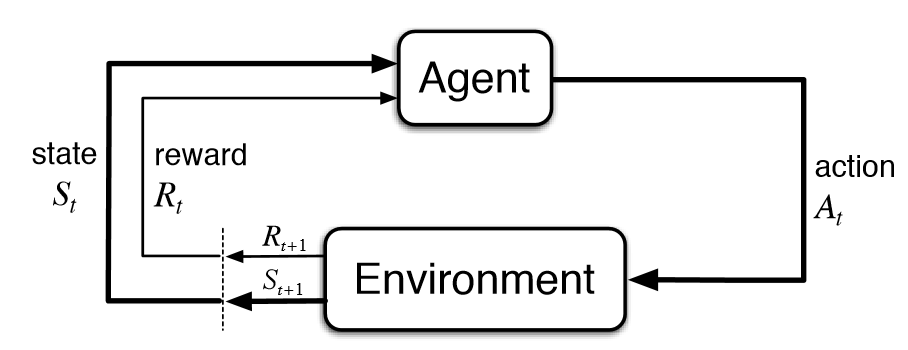
\includegraphics[width=0.7\textwidth]{figs/rl.png}
    \caption{Reinforcement Learning\protect\footnotemark[1]}
    \label{fig:rldiag}
\end{figure}
\footnotetext[1]{
\hyperlink{https://towardsdatascience.com/reinforcement-learning-101-e24b50e1d292}
{https://towardsdatascience.com/reinforcement-learning-101-e24b50e1d292}}

% \begin{quote}
%     Some key terms that describe the basic elements of an RL problem are\footnotemark[1]:
%     \begin{itemize}
%         \item Environment: Physical world in which the agent operates
%         \item State: Current situation of the agent
%         \item Reward: Feedback from the environment
%         \item Policy: Method to map agent’s state to actions
%         \item Value: Future reward that an agent would receive by taking an action in a particular state
%     \end{itemize}
% \end{quote}

Compared with supervised learning, the reward in RL may only be given occasionally and summarily
(e.g. if the agent eventually reaches a desired state after a path of actions)

\subsection{Data}

Common datasets (Benchmark):
\begin{itemize}
    \item small image datasets: MNIST [1,28,28] (extend to EMNIST, fashion-MNIST), CIFAR-10 [3,32,32];
    \item large image datasets: ImageNet [3,256,256];
    \item text datasets for text classification: IMDB movie review dataset;
    \item text datasets for machine translation: documents from multilingual organizations 
    (e.g. Canadian parliament and EU), WMT dataset;
    \item seq2seq tasks (e.g. document summarication and question answering): ?.
\end{itemize}

\textbf{TF-IDF}: term frequency-inverse document frequency.\unsure{
weighted BoW that reduce the importance of uninformative terms
}
TF$_{ij}$ is the frequency of term $i$ in document $j$, and 
IDF$_i\triangleq{\frac{N}{1+\text{DF}_i}}$, 
where $DF_i$ is the number of documents with term $i$.
\begin{gather}
    \text{TF-IDF}_{ij}=\log{\text{TF}_{ij}+1}\times\text{IDF}_i
\end{gather}

\textbf{Word embeddings}: 
\unsure{
Usually self-supervised models were adopted to build a pre-trained word embeddings 
based on large-scale contexts.
}\unsure{
The embeddings with similar meanings be often close in some metric space.}
map sparse and vocabulary-length (high-dimensional) vectors to 
dense and low-dimensional ones (embeddings).

Strategies to deal with OOV:
\begin{enumerate}
    \item replace all novel words with $\mathtt{UNK}$;
    \item byte-pair encoding: finer-grained subword structure embedding;
\end{enumerate}

Let $\bm{M}\in\mathbb{I}^{N\times{D}}$ indicates the missing status of feature $\bm{X}$:
$M_{nd}=1$ if $X_{nd}$ is missing and let $\bm{X}_v~(\bm{M}_v=\bm{0})$ and 
$\bm{X}_h~(\bm{M}_h=\bm{1})$ 
are visible and missing parts of features, respectively. 
The outcome labels $\mathbf{Y}$ are full observed.\unsure{
Missing data handling is a complex topic,
also important in \textit{clinical trial designing}, 
and will be discussed later and further.
}
\begin{itemize}
    \item \textbf{missing completely at random} (MCAR): 
    $p(\bm{M}|\bm{X}_v,\bm{X}_h,\bm{Y})=p(\bm{M})$,
    the missingness does not depend on the hidden/observed features;
    \item \textbf{missing at random} (MAR):
    $p(\bm{M}|\bm{X}_v,\bm{X}_h,\bm{Y})
    =p(\bm{M}|\bm{X}_v,\bm{Y})$,
    the missingness does not depend on the hidden features but may depend on the visible features;
    \item \textbf{not missing at random} (NMAR): otherwise
\end{itemize}

\begin{note}
    In the MCAR/MAR case, the missingness mechanism can be ignored since missingness is
    independent with the unobserved features. 
    And \textbf{this book always makes the MAR assumption}.
\end{note}

\section{Foundations}
\begin{quote}
    \citep{pml1Book} -- Chapter 2-8.
\end{quote}

\subsection{Probability: Univariable and Multivariable Models}

Types of uncertainty:
\begin{enumerate}
    \item \textbf{model uncertainty}: or epistemic uncertainty,
    caused by our ignorance of the underlying hidden causes or mechanism generating the data;
    \item \textbf{data uncertainty}: or aleatoric uncertainty,
    caused by intrinsic variability (the true model generating data randomly).
\end{enumerate}

Paradigm of binary classification with the assumption of probability output:
\begin{gather}
    p(y|\bm{x},\bm{\theta})
    =\text{Bernoulli}(y|\sigma(f(\bm{x};\bm{\theta})))
\end{gather}
where basic property of neuron, activation function $\sigma(a)$, in a network's output layer is compressing the value of unconstrained function to $[0,1]$, 
one example with good characteristics (refer to \citep{pml1Book} Table 2.3) 
of which is the sigmoid function $\frac{1}{1+e^{-a}}$, 
and the variety of $f$'s contributes to the contemporary blossom of deep learning architectures, 
the easiest one of which is linear model $\bm{w}^T\bm{x}+b$. (Logistic regression: Binomial+Sigmoid \& Multinomial+Softmax
\unsure{log-sum-exp trick for computer friendly to avoid floating-point overflow})

Paradigm of regression:
\begin{gather}
    p(y|\bm{x};\bm{\theta})
    =\mathcal{N}(y|
    f_\mu(\bm{x};\bm{\theta}),
    f_\sigma^2(\bm{x};\bm{\theta})
    )
\end{gather}
where $f_\mu\in\mathbb{R}$ predicts the mean 
and $f_\sigma^2\in\mathbb{R}^+$ predicts the variance.
Recall the two types of uncertainty,
the \textbf{uncertainty of data} ($y$) is presented by $f_\sigma(\bm{x};\bm{\hat{\theta}})$ and 
the \textbf{uncertainty of model} ($\bm{\theta}$) is presented by 
$\mathrm{Var}f_\mu(\bm{x};\bm{\theta})$.

Gaussian (or Normal) distribution has good characteristics
\begin{enumerate}
    \item with two parameters $\mu,\sigma^2$, easy to interpret;
    \item by central limit theorem (modeling the noise from multiple sources);
    \item with the least number of assumptions;
    \item with simple form, easy to implement but highly effective.
\end{enumerate}

\textbf{Heavy-tail} distributions, say, 
Student, Cauchy, and Laplace (double sided Exp.) distributions, 
is robust to outliers.\unsure{
Grafting of Normal main body and Cauchy tails are also used to deal with outliers like RCTD.
} 
It is common to set $\nu=4$, if greater, then Student dist. approaches to $\mathcal{N}$.

\textbf{Monte Carlo approximation}. 
Consider an arbitrary transformation $\bm{Y}=g(\bm{X})$,
it is often difficult to compute the induced distribution $f_{\bm{Y}}(\bm{y})$ analytically,
but it can be approached by drawing a large amount of samples 
from the original distribution $f_{\bm{X}}(\bm{x})$:
\begin{gather}
    f_{\hat{\bm{Y}}}(\bm{y})
    \triangleq
    \frac{1}{N}\sum_{s=1}^N\delta(\bm{y}-g(\bm{x}_s))
\end{gather}



% \begin{framed}{\Large

% TODO list in the following week
% \begin{itemize}
%     \item Finish reading the remaining chapters in the Foundation part
%     \item Finish reading \citep{shao2003mathematical} and 
%     do the exercises (for STAT5005)
%     \item Finish organizing the hand writing notes of STAT5010.
% \end{itemize}

% }\end{framed}
\textbf{Simpson's paradox} says that a statistical trend or relationship 
that appears in several difficult groups of data can disappear or reverse sign 
when these groups are combined.

\textbf{Convariance} of multiple r.v.. $\bm{X}=(X_1,\cdots,X_D)$ is defined as\unsure{
Useful in Multivariate Analysis and Linear Model
} 
\begin{align}
    \bm{\Sigma}\triangleq\mathrm{Cov}\bm{X}
    =& \mathbb{E}\left[
    (\bm{X}-\mathbb{E}\bm{X})
    (\bm{X}-\mathbb{E}\bm{X})^T
    \right]\\
    =& \mathbb{E}[\bm{XX}^T]-[\mathbb{E}\bm{X}][\mathbb{E}\bm{X}]^T
\end{align}
\begin{enumerate}
    \item $\mathbb{E}[\bm{XX}^T]=\bm{\Sigma}+\bm{\mu}\bm{\mu}^T$
    \item $\mathrm{Cov}[\bm{AX}+\bm{b}]=\bm{A}\mathrm{Cov}\bm{X}\bm{A}^T$
    \item \improvement{There are some other properties of multiple r.v. waiting to be added.}
\end{enumerate}

\textbf{Multivariate Gaussian/normal} (MVN) r.v. 
$\bm{X}\sim\mathcal{N}(\bm{\mu},\bm{\Sigma})$
\begin{gather}
    f_{\bm{X}}(\bm{x})
    = \frac{1}{(2\pi)^\frac{D}{2}|\bm{\Sigma}|^\frac{1}{2}}
    \exp\left\{ 
        -\frac{1}{2}
        (\bm{x}-\bm{\mu})^T
        \bm{\Sigma}^{-1}
        (\bm{x}-\bm{\mu}) 
    \right\}
\end{gather}

\textbf{Mahalanobis distance} $\Delta$ between $\bm{x}$ and $\bm{\mu}$
under the assumption of above MVN is defined as
\begin{gather}
    \Delta^2\triangleq
    (\bm{x}-\bm{\mu})^T
    \bm{\Sigma}^{-1}
    (\bm{x}-\bm{\mu}),
\end{gather}
implying that \uline{the points with a same density have a same Mahalanobis distance 
away from the population mean point $\bm{\mu}$}, say, like contours.
It can be interpreted as Euclidean distance in a new coordinate 
from the original coordinate by the transformation of 
$\bm{\Sigma}^{-1}$,
which can be computed by eigendecomposition:
\begin{gather}
    \bm{\Sigma}
    = \sum_{d=1}^D{\lambda_d\bm{u}_d\bm{u}_d^T}
    % = \bm{U}\mathrm{diag}(\lambda_1,\cdots,\lambda_D)\bm{U}^T\\
    = \bm{U}\bm{D}\bm{U}^T\\
    \bm{\Sigma}^{-1}
    = \sum_{d=1}^D{\lambda_d^{-1}\bm{u}_d\bm{u}_d^T}
    % = \bm{U}\mathrm{diag}(\lambda_1,\cdots,\lambda_D)^{-1}\bm{U}^T
    = \bm{U}\bm{D}^{-1}\bm{U}^T
    \triangleq \bm{\Lambda}
\end{gather}
where $\bm{U}=[\bm{u}_1,\cdots,\bm{u}_D]$ is eigenvectors for rotation and 
$\bm{D}=\mathrm{diag}(\lambda_1,\cdots,\lambda_D)$ is eigenvalues for scaling.\unsure{
This procedure is similar with the standardization of univariable Gaussian.}


\textbf{Marginals and conditionals of an MVN}: \info{
Marginals and conditionals of a multi-variable model is important and frequently used conclusion.
}
Suppose $\bm{X}=[\bm{X}_1,\bm{X}_2]^T\sim\mathcal{N}(\bm{\mu},\bm{\Sigma})$, where
\begin{gather}
    \bm{\mu}=\left[\begin{array}{c}
        \bm{\mu}_1 \\
        \bm{\mu}_2
    \end{array}\right],~
    \bm{\Sigma}=\left[\begin{array}{cc}
        \bm{\Sigma}_{11} & \bm{\Sigma}_{12} \\
        \bm{\Sigma}_{21} & \bm{\Sigma}_{22}
    \end{array}\right],~\text{and}~
    \bm{\Lambda}
    =\bm{\Sigma}^{-1}=\left[\begin{array}{cc}
        \bm{\Lambda}_{11} & \bm{\Lambda}_{12} \\
        \bm{\Lambda}_{21} & \bm{\Lambda}_{22}
    \end{array}\right]
\end{gather}
is the \textbf{precision matrix}.
$\Rightarrow$
\begin{align}
    \bm{X}_1
    \sim& \mathcal{N}(\bm{\mu}_1,\bm{\Sigma}_{11}),\\
    \bm{X}_1|\bm{X}_2
    \sim& \mathcal{N}
    (\bm{\mu}_{1|2},\bm{\Sigma}_{1|2})
\end{align}
where 
\begin{align}
    \bm{\mu}_{1|2}
    =& \bm{\Sigma}_{1|2}
    [\bm{\Lambda}_{11}\bm{\mu}_1
    -\bm{\Lambda}_{12}(\bm{X}_2-\bm{\mu}_2)],\\
    \bm{\Sigma}_{1|2}
    =& \bm{\Sigma}_{11}
    -\bm{\Sigma}_{12}\bm{\Sigma}_{22}^{-1}\bm{\Sigma}_{21}
    =\bm{\Lambda}_{11}^{-1}.
\end{align}

% \begin{example}
%     $~$\\
%     $\bm{\Sigma}=\left[\begin{array}{cc}
%         \sigma_1^2 & \rho\sigma_1\sigma_2 \\
%         \rho\sigma_1\sigma_2 & \sigma_2^2
%     \end{array}\right]$, and compute the marginal and conditional distribution.
% \end{example}

\begin{example}
    \textbf{Missing value imputation}\\
    infer the missing entries 
    by exploiting the correlation (in $\bm{\Sigma}$) amongst the dimensions,
    say, computing 
    $p(\bm{x}_{n,\bm{h}}|\bm{x}_{n,\bm{v}},\bm{\theta})$
    and obtain the posterior mean (optimally guessed values) and variance (confidence measure).
\end{example}


\textbf{Linear Gaussian system}.
Let $\bm{Z}\in\mathbb{R}^L$ be an unknown vector of values, 
and $\bm{Y}\in\mathbb{R}^D$ be some \textbf{noisy measurement} of $\bm{Z}$:
\begin{align}
    \bm{Z}
    \sim& \mathcal{N}(\bm{\mu}_z,\bm{\Sigma}_z)\\
    \bm{Y}|\bm{Z}=\bm{z}
    \sim& \mathcal{N}(\bm{Wz}+\bm{b},\bm{\Sigma}_y)
\end{align}
The joint distribution of $[\bm{Z},\bm{Y}]$ follows is Gaussain 
$\mathcal{N}(\bm{\mu},\bm{\Sigma})$, where\unsure{
The unconditional variance of $\bm{Y}$ includes its conditional variance, $\bm{\Sigma}_y$,
and the squared weight-scaled variance of $\bm{Z}$, $\bm{W\Sigma}_z\bm{W}^T$.
}
\begin{gather}
    \bm{\mu}
    = \left[\begin{array}{c}
        \bm{\mu}_z \\
        \bm{W\mu}_z+\bm{b} 
    \end{array}\right],~
    \bm{\Sigma}
    = \left[\begin{array}{cc}
        \bm{\Sigma}_z & \bm{\Sigma}_z\bm{W}^T \\
        \bm{W\Sigma}_z & \bm{\Sigma}_y+\bm{W\Sigma}_z\bm{W}^T
    \end{array}\right]
\end{gather}

\begin{example}
    \textbf{relationship from observations to latent factors}\\
    Infer the \uline{relationship from observations to latent factors}: $\bm{Y}\to\bm{Z}$ by Bayes rule:
    \begin{align}
        \bm{Y}
        \sim& \mathcal{N}(\bm{W\mu}_z+\bm{b},\bm{\Sigma}_y+\bm{W\Sigma}_z\bm{W}^T)\\
        \bm{Z}|\bm{Y}=\bm{y}
        \sim& \mathcal{N}(\bm{\mu}_{z|y},\bm{\Sigma}_{z|y}),
    \end{align}
    where
    \begin{align}
        \bm{\mu}_{z|y}
        =& \bm{\Sigma}_{z|y}\left[
            \bm{W}^T\bm{\Sigma}_y^{-1}(\bm{y}-\bm{b})+\bm{\Sigma}_z^{-1}\bm{\mu}_z
        \right]~\text{and}~\\
        \bm{\Sigma}_{z|y}^{-1}
        =& \bm{\Sigma}_z^{-1}+\bm{W}^T\bm{\Sigma}_y^{-1}\bm{W}
    \end{align}
\end{example}

\begin{example}
    \textbf{shrinkage} and \textbf{Singal-to-noise ratio}\\
    Suppose $Y_i=Z+\varepsilon$ is the observed signal with 
    $\varepsilon\sim\mathcal{N}(0,\Sigma_y)$ and
    $Y_i|Z=z\sim\mathcal{N}(z,\Sigma_y)$,
    and $z\sim\mathcal{N}(\mu_0,\Sigma_0)$ is the true signal, 
    then $Z|\bm{y}\sim\mathcal{N}(\mu_N,\Sigma_N)$, where
    \begin{align}
        \Sigma_N
        =& \left(\Sigma_0^{-1}+N\Sigma_N^{-1}\right)^{-1}\\
        \mu_N
        % =& \frac{\Sigma_y/N}{\Sigma_0+\Sigma_y/N}\mu_0+\frac{\Sigma_0}{\Sigma_0+\Sigma_y/N}\Bar{y}_N\\
        % =& \mu_0 + ({\Bar{y}_N-\mu_0})\frac{\Sigma_0}{\Sigma_y/N+\Sigma_0}\\
        =& \Bar{y}_N - (\Bar{y}_N-\mu_0)\frac{\Sigma_y/N}{\Sigma_y/N+\Sigma_0} \label{eq:shrinkage}
    \end{align}
    The data is adjusted towards the prior mean with the increasing of noise deviation, called \textbf{shrinkage}, by Equation (\ref{eq:shrinkage}).
    And the amount of shrinkage is defined as \textbf{signal-to-noise ratio}, 
    \begin{gather}
        \text{SNR}\triangleq\frac{\mathbb{E}Z^2}{\mathbb{E}\varepsilon^2}=\frac{\Sigma_0+\mu_0^2}{\Sigma_y}
    \end{gather}
    By increasing the number of observations, 
    the SNR can be amplified through reducing the variance of noise $\varepsilon$, 
    and this conclusion can be extend to multi-variable case.
\end{example}
% \unsure{
%     recall the convex combination of the prior and the data
%     }
\begin{example}
    \textbf{Senser fusion}\\
    There are $M$ sensors (measurement devices) and $N_m$ observations for each devices, 
    the the signals $Y_{1,m},\cdots,Y_{n,m},\cdots,Y_{N_m,m}|\bm{Z}=\bm{z}\overset{iid}{\sim}\mathcal{N}(\bm{z},\Sigma_m)$. Sensor fusion is to combine the evidence together, to compute $p(\bm{z}|\bm{y})$.
\end{example}

\begin{question}
    Why is exponential family so important?
\end{question}

\textbf{Maximum entropy derivation of the exponential family}:
Recall \textbf{KL divergence} of two distributions, $p$ and $q$, not symmetric
\begin{gather}
    \infdiv{p}{q}
    \triangleq\left\{
    \begin{array}{ll}
        \int_\mathcal{X}{p(x)\log\frac{q(x)}{p(x)}}dx & X~\text{continuous} \\
        \sum_x{p(x)\log\frac{p(x)}{q(x)}} & X~\text{discrete}
    \end{array}\right.
\end{gather}
To find a distribution $p$ that minimizes the $\infdiv{p}{q}$ with a given priori $q$
with moments constraints of observed data
\begin{gather}
    p^*=\argmin_p\infdiv{p}{q}\\
    \mathrm{s.t.}~\sum_x{p(x)}=1
    ~\text{and}~
    \sum_x{p(x)f_k(x)}=F_k,~k=1,\cdots,K
\end{gather}
The Lagrangian is given by
{\small\begin{gather}
    J(p,\bm{\lambda})
    =- \sum_x{p(x)\log\frac{p(x)}{q(x)}}
    + \lambda_0\left[1-\sum_x{p(x)}\right]
    + \sum_k{\lambda_k\left[ F_k-\sum_x{p(x)f_k(x)} \right]}\\
\Rightarrow
    p^*(x)=\frac{1}{Z}q(x)\exp\left\{-\sum_k{\lambda_kf_k(x)}\right\}
\end{gather}}
which is exactly the form of exponential family and where $Z$ is the normalization term.
e.g. if $f_1(x)=x$ and $f_2(x)=x^2$, then the best distribution with minimum KL divergence 
(or maximum entropy) and matching the observed first and second moments is Gaussian distribution.

\textbf{Gaussain mixture model} (GMM) or \textbf{mixture of Gaussian} (MoG): 
the probability of each data point $\bm{y}_n$\unsure{
Are the proportion $\pi_k$'s different for each data points?
What is the relationship between $r_{nk}$ and $\pi_k$ in Equation (\ref{eq:mogpir})?
} is determined 
by certain weights of multiple distinct Gaussian models,
often used for clustering, e.g. K-means with $\bm{\Sigma}_k=\bm{I}$, $k=1,\cdots,K$.
\begin{gather}
    p(\bm{y}|\bm{\theta})=\sum_{k=1}^K{\pi_k\mathcal{N}(\bm{\mu}_k,\bm{\Sigma}_k)}
\end{gather}
\begin{align}
    \hat{\bm{\theta}}
    =& \argmax_{\bm{\theta}}\log{p(\bm{y}_1,\cdots,\bm{y}_N|\bm{\theta})}~\text{(by MLE)}\\
    \hat{\pi}_{nk}
    \overset{?}{=}& r_{nk}\triangleq p(z_n=k|\bm{y}_n,\hat{\bm{\theta}}) \label{eq:mogpir}\\
    =& \frac{p(z_n=k|\hat{\bm{\theta}})p(\bm{y}_n|z_n=k,\hat{\bm{\theta})z}}
    {\sum_{k'=1}^K{p(z_n=k'|\hat{\bm{\theta}})p(\bm{y}_n|z_n=k',\hat{\bm{\theta})}}}~\text{(by Bayes)}
\end{align}
\improvement{
The optimization process of EM or SGD will be discussed in \citep{pml1Book}, Chapter 8.
}

\textbf{Bernoulli mixture model} (BMM) or \textbf{mixture of Bernoullis} (MoB):
similar with MoG:
\begin{gather}
    p(\bm{y}|\bm{\theta})=\sum_{k=1}^K{\pi_k\underbrace{\prod_{d=1}^D\mathrm{Ber}(y_d|\mu_{dk})}_{\text{proba. of r. vec.}}}
\end{gather}

\textbf{Ordered Markov property} in a \textbf{Bayesian network} is that 
each node $Y_i$ is conditionally independent of all its predecessors ($\bm{Y}_{\text{pre}(i)}$) given its parents ($\bm{Y}_{\text{par}(i)}$):
\begin{gather}
    Y_i\perp\bm{Y}_{\text{pre}(i)\setminus\text{par}(i)}|\bm{Y}_{\text{par}(i)}\\
    p(\bm{Y}_{1:N_G})=\prod_{i=1}^{N_G}p\left(Y_i|\bm{Y}_{\text{par}(i)}\right)
\end{gather}
where $p\left(Y_i|\bm{Y}_{\text{par}(i)}\right)$ is called \textbf{conditional probability distribution} (CPD), 
which can be written as the conditional probability table (CPT) 
when the status of each node is (discrete) categorical distribution.
In Markov chain model, 
$p(y_t|y_{t-1})$ is called \textbf{transition function/kernel} (or \textbf{state transition matrix} in the case of discrete status) and is \textbf{stationary/time-invariant} under the assumption that $p(y_t|y_{t-1})$ is the same for all time steps.

\begin{figure}[hptb]
    \centering
    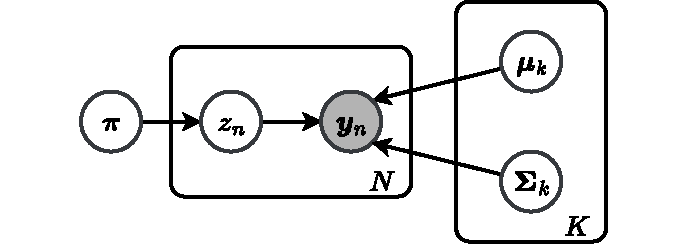
\includegraphics[width=0.5\textwidth]{figs/mixgaussian.pdf}
    \caption{A Gaussian mixture model represented as a graphical model}
    \label{fig:maxgaussian}
\end{figure}

\begin{example}
    \textbf{GMM represented as a graphical model}\\
    Viewing all variables, including model's parameters and obverations, 
    follow a generative story like Figure (\ref{fig:maxgaussian})
    {\small\begin{gather}
        p(\bm{y}_{1:N},\bm{z}_{1:N},\bm{\theta})
        = p(\bm{pi})
        \left[ \prod_{k=1}^K p(\bm{\mu}_k)p(\bm{\Sigma}_k) \right]
        \left[ \prod_{n=1}^N p(z_n|\bm{\pi})p(\bm{y}_n|z_n,\bm{\mu}_{1:K},\bm{\Sigma}_{1:K}) \right]
    \end{gather}}
    where latent variable $z_n\sim\text{Cat}(\bm{\pi})$ and model's parameters
    $\bm{\theta}=(\bm{\pi},\bm{\mu}_{1:K},\bm{\Sigma}_{1:K})$ are all unknown.
\end{example}



% \begin{framed}{\large
% TODO list in the following week
% \begin{itemize}
%     \item Finish reading the remaining chapters in the Foundation part
%     \item Finish reading \citep{shao2003mathematical} and 
%     do the exercises (for STAT5005)
%     \item Finish organizing the hand writing notes of STAT5010.
% \end{itemize}
% }\end{framed}




% ############################### WK 2 #######################################

% \setcounter{section}{2}
% \setcounter{subsection}{2}
% \begin{center}
% \textit{Continue Chapter 2 \& 3 univariate and multivariate models}
% \end{center}

% \subsection{Statistics}

\begin{question}
    Why can MLE be used so uniformly?
\end{question}

\textbf{Maximum likelihood estimation} (MLE) and \textbf{maximum a posterior estimation} (MAP):
$\hat{\bm{\theta}}_{MLE}$ -- the parameters' estimation that assign the highest probability to the observations;
$\hat{\bm{\theta}_{MAP}}$ -- the parameters' estimation maximizing the posterior probability under some priori $\pi(\bm{\theta})$. 
If \uline{the priori is a uniform distribution}, 
then $\hat{\bm{\theta}}_{MLE}=\hat{\bm{\theta}}_{MAP}$.\unsure{
Reason 1
}
\begin{gather}
    \hat{\bm{\theta}}_{MLE}
    \triangleq \argmax_{\bm{\theta}}p(\mathcal{D}|\bm{\theta})\\
    \hat{\bm{\theta}}_{MAP}
    \triangleq \argmax_{\bm{\theta}}p(\bm{\theta}|\mathcal{D})
    = \argmax_{\bm{\theta}}p(\mathcal{D}|\bm{\theta})\pi(\bm{\theta})
\end{gather}
\textbf{Kullback Leibler divergence} (KL divergence): 
A standard way to measure the dissimilarity between probability distribution $p$ and $q$.
\begin{align}
    \infdiv{p}{q}
    =& \sum_{\bm{y}}{p(\bm{y})\log\frac{p(\bm{y})}{q(\bm{y})}}\\
    =& \underbrace{\sum_{\bm{y}}{p(\bm{y})\log p(\bm{y})}}_{-\mathbb{H}(p)\text{:entropy}}
    - \underbrace{\sum_{\bm{y}}{p(\bm{y})\log q(\bm{y})}}_{-\mathbb{H}_{\text{CE}}(p,q)\text{:cross-entropy}}
\end{align}
If \uline{$q(\bm{y})=p(\bm{y}|\bm{\theta})$ and $p(\bm{y})=p_\mathcal{D}(\bm{y})$}, 
then $\infdiv{p}{q}=\text{const}+\mathrm{NNL}(\bm{\theta})$.\unsure{Reason 2}
which shows the relationship between MLE and KL divergence.
And above all justify usage of MLE from the perspectives of Bayesain and empirical distribution.

\begin{example}
    \textbf{MLE for linear regression} aka\\
    \textbf{ordinary least squares} or OLS estimate
    \begin{align}
        p(y|\bm{x};\bm{\theta})
        =& \mathcal{N}(\bm{w}^T\bm{x},\sigma^2)\\
        \hat{\bm{w}}_{OLS}\equiv\hat{\bm{w}}_{MLE}
        \triangleq& \argmin_{\bm{w}}\text{NLL or RSS or MSE or RMSE}\\
        =& (\bm{X}^T\bm{X})^{-1}\bm{X}^T\bm{y}
    \end{align}
\end{example}

\textbf{Empirical risk minimization} (ERM) 
\begin{gather}
    \mathcal{L}(\bm{\theta})=\frac{1}{N}\sum_{n=1}^N\ell(\bm{y}_n,\bm{\theta};\bm{x}_n)
\end{gather}
where $\ell(\cdot)$ is any loss function that measures the mismatchness with expected outcomes, 
(if $\ell(\bm{y}_n,\bm{\theta};\bm{x}_n)=-\log{p(\bm{y}_n|\bm{\theta},\bm{x}_n)}$,
then $\mathcal{L}(\bm{\theta})=\text{NLL}(\bm{\theta})$ and ERM is MLE).\unsure{Reason 3}
% \textbf{Surrogate loss function}: 
% The surrogate is usually chosen to be a maximally tight
% convex upper bound, which is then easy to minimize, e.g. 

% \begin{enumerate}[(i)]
%     \item 0-1 loss: 
%     $\ell_{01}(\bm{y}_n,\bm{\theta};\bm{x}_n)=\mathbb{I}(\bm{y}_n\neq f(\bm{x}_n;\bm{\theta})$
%     \item :
    
% \end{enumerate}

\begin{figure}[hptb]
    \centering
    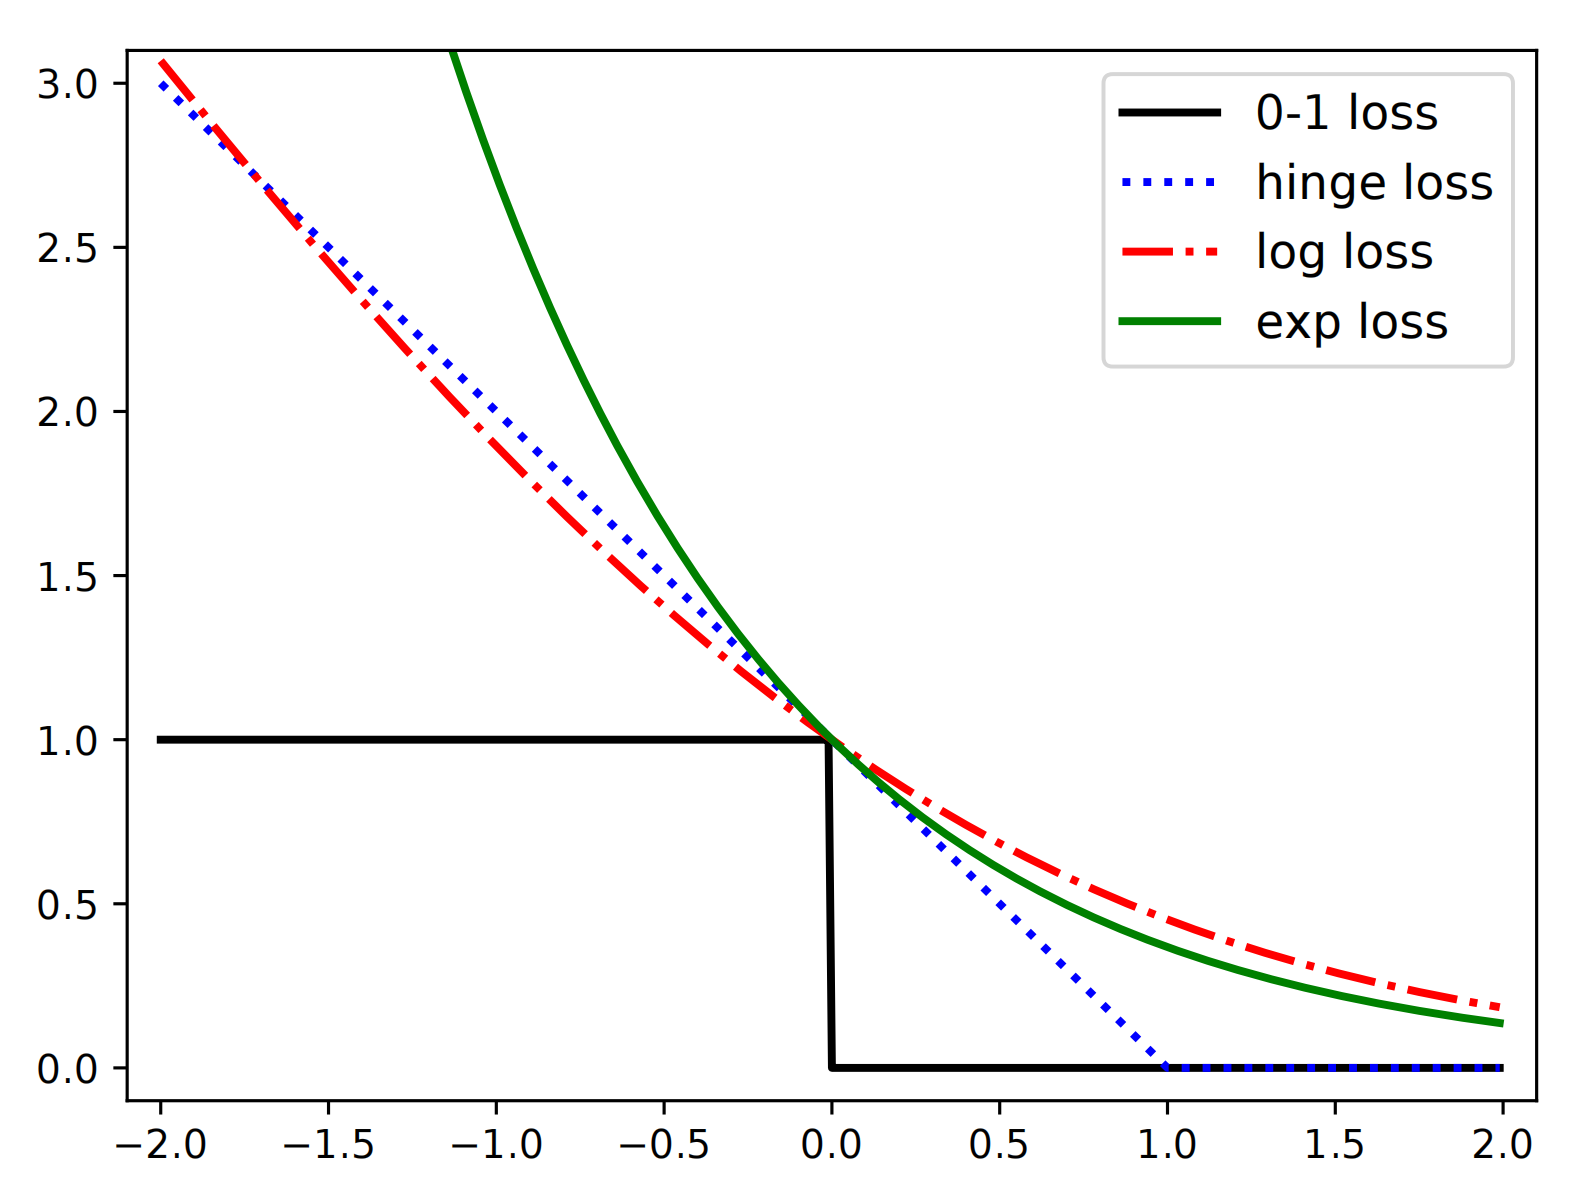
\includegraphics[width=0.5\textwidth]{figs/lossfunc.png}
    \caption{Loss functions for \uline{binary classifiers}}
    {\footnotesize Horizontal axis: $z=yf(\bm{x};\bm{\theta})$. \\
    0-1 loss: $\mathbb{I}(z<0)$;
    Hinge loss: $\max\{0,1-z\}$;
    Log-loss: $\log_2{(1+e^{-z})}$;
    Exp-loss: $e^{-z}$.}
    \label{fig:lossfunc}
\end{figure}

\textbf{Estimation method of moments} (MOM): 
equate the \uline{theoretical moments (functions of parameters)},
to the \uline{empirical moments},
where we need the same number of simultaneous equations for solving $K$ unknown parameters,
to avoid difficult computation in MLE 
but with less efficiency of data usage, so can be used to initialize iterative algorithms for MLE.

\textbf{Online (recursive) estimation} with recursive update $f$:
\begin{gather}
    \hat{\bm{\theta}}_t=f(\hat{\bm{\theta}}_{t-1},\bm{y}_t)
\end{gather}

\begin{example}
    \textbf{Exponentially-weighted moving average} (EWMA)
    \begin{align}
        \hat{\bm{\mu}}_t
        =& \beta\hat{\bm{\mu}}_{t-1}+(1-\beta)\hat{\bm{y}}_t\\
        =& \beta^t\bm{y}_0 + (1-\beta)\beta^{t-1}\bm{y}_1 + \cdots + (1-\beta)\beta\bm{y}_{t-1} + (1-\beta)\bm{y}_t
    \end{align}
    where a smaller $\beta$ forgets the past data more quickly and 
    adapts to the more recent data more rapidly.
\end{example}

\textbf{Regularization} term $C(\bm{\theta})$ in the loss function is 
a given measure for the parameters' complexity to avoid overfitting:
\begin{gather}
    \mathcal{L}(\bm{\theta};\lambda)
    = \frac{1}{N}\sum_{n=1}^N\ell(\bm{y}_n,\bm{\theta};\bm{x}_n)
    + \lambda C(\bm{\theta})
\end{gather}
where $C(\bm{\theta})$ can be some $-\log{\pi(\bm{\theta})}$,
then objective become a MAP estimation for a given priori $\pi(\bm{\theta})$ for $\lambda=1$.
e.g. add-one smoothing (or \textbf{Laplace's rule of succession}) in Bernoulli distribution with $\pi\sim\text{Beta}(2,2)$ $p\sim$ and shrinkage estimation for $\Sigma$ in multivariate Gaussian with $\pi\sim$ inverse Wishart. 

\textbf{Bayes model averaging} (BMA): make predictions under the posterior distribution of parameters, which weighted the predictions for all possible parameters (models)
\begin{gather}
    \pi(\bm{\theta}|\mathcal{D})
    = \frac{\pi(\bm{\theta})p(\mathcal{D}|\bm{\theta})}{p(\mathcal{D})}\\
    p(\bm{y}|\bm{x},\mathcal{D})
    = \int{p(\bm{y}|\bm{x};\bm{\theta})\pi(\bm{\theta}|\mathcal{D})}d\bm{\theta}
\end{gather}
where $\bm{x}$ is new observations, $\mathcal{D}$ is training data, and 
$p(\bm{y}|\bm{x},\mathcal{D})$ is the final averaging model.


\textbf{Mixtures of priors} by introducing a latent indicator variable $h$
\begin{gather}
    \pi(\bm{\theta})=\sum_k p(h=k)\pi(\bm{\theta}|h=k)
\end{gather}
$\Rightarrow$
\begin{align}
    \pi(\bm{\theta}|\mathcal{D})
    =& \sum_k{p(h=k|\mathcal{D})p(\bm{\theta}|\mathcal{D},h=k)}\\
    p(h=k|\mathcal{D})
    =& \frac{p(h=k)p(\mathcal{D}|h=k)}{\sum_{k'}{p(h=k')p(\mathcal{D}|h=k')}}
\end{align}
\improvement{
The detailed discussion on 
prior, posterior, predictive, and marginal likelihood of
(1) Beta-Binomial, (2)\textbf{Dirichlet-Multinomial}, and (3) Gaussian-Gaussian
are skipped.
}

\textbf{Other priors} besides conjugate priors
\begin{enumerate}[(1)]\label{kspt:noninfo}
    \item \textbf{noninformative prior} or preferred \textbf{minimally informative prior}: 
    let the data speak for itself, 
    e.g. \textbf{flat prior} $\pi\propto 1$ in Gaussian;
    \item \textbf{hierarchical prior}: the hyperparameters in prior also follow some prior --
    $\bm{\phi}\to\bm{\theta}\to\mathcal{D}$;
    \item \textbf{empirical prior}: the prior's hyperparameters $\bm{\phi}$ directly estimated from data $\mathcal{D}$ as shown below
    \begin{gather}
        \hat{\bm{\phi}}(\mathcal{D})
        = \argmax_{\bm{\phi}}p(\mathcal{D}|\bm{\phi})
        = \argmax_{\bm{\phi}}\int{p(\mathcal{D}|\bm{\theta})p(\bm{\theta}|\bm{\phi})}d\bm{\theta}
    \end{gather}
    which is called \textbf{Empirical Bayes} (EB).
\end{enumerate}

Available inference methods:
\begin{itemize}
    \item MLE:
    \begin{gather}
        \hat{\bm{\theta}}
    =\argmax_{\bm{\theta}}
    p(\mathcal{D}|\bm{\theta})
    \end{gather}
    \item MAP: 
    \begin{gather}
        \hat{\bm{\theta}}
    =\argmax_{\bm{\theta}}
    p(\mathcal{D}|\bm{\theta})p(\bm{\theta}|\bm{\phi})
    \end{gather}
    \item MLE-II (EB):
    \begin{gather}
        \hat{\bm{\phi}}
    =\argmax_{\bm{\phi}}
    \int{p(\mathcal{D}|\bm{\theta})p(\bm{\theta}|\bm{\phi})}d\bm{\theta}
    \end{gather}
    \item MAP-II:
    \begin{gather}
        \hat{\bm{\phi}}
    =\argmax_{\bm{\phi}}
    \int{p(\mathcal{D}|\bm{\theta})p(\bm{\theta}|\bm{\phi})p(\bm{\phi})}d\bm{\theta}
    \end{gather}
    \item Full Bayes:
    \begin{gather}
        p(\bm{\theta},\bm{\phi}|\mathcal{D})
    \propto p(\mathcal{D}|\bm{\theta})p(\bm{\theta}|\bm{\phi})p(\bm{\phi})
    \end{gather}
\end{itemize}

\textbf{Computational issues} in Bayesian ML: 
It is usually \uline{intractable to compute $p(\bm{\theta}|\mathcal{D})$}
given $p(\mathcal{D}|\bm{\theta})$ and $p(\bm{\theta})$.
Therefore, methods of \textbf{approximate posterior inference} are necessary.
\begin{itemize}
    \item \textbf{Grid approximation}:  
    brute-force enumerate finite set in partition the space of possible values $\bm{\theta}$.
    \begin{gather}
        p(\bm{\theta}=\bm{\theta}_k|\mathcal{D})
        \approx \frac{p(\mathcal{D}|\bm{\theta}_k)}{\sum_{k'=1}^K{p(\mathcal{D},\bm{\theta}_{k'})}}
    \end{gather}
    \item \textbf{Quadratic (Laplace) approximation}: 
    approximate the posterior by a multivariable Gaussian.
    $\mathcal{E}(\bm{\theta})=-\log{p(\bm{\theta},\mathcal{D})}$ is an \textbf{energy function}, 
    $\hat{\bm{\theta}}$ is the mode ($\Rightarrow\nabla{\mathcal{E}(\bm{\theta})}|_{\bm{\theta}=\hat{\bm{\theta}}}=\bm{0}$), 
    at which $\mathbf{H}$ is Hessian of $\mathcal{E}$.
    \begin{gather}
        p(\bm{\theta}|\mathcal{D})
        \approx \mathcal{N}(\hat{\bm{\theta}},\mathbf{H}^{-1})
    \end{gather}
    \item \textbf{Variational approximation}: 
    find a $q$ minimizing \uline{some discrepancy $D$}, say KL divergence, with target posterior
    in tractable family of distribution $\mathcal{Q}$,
    \begin{gather}
        p(\bm{\theta}|\mathcal{D})
        \approx q^*=\argmin_{q\in\mathcal{Q}} \infdiv{q}{p}
    \end{gather}
    \item \textbf{Monte Carlo approximation}: 
    build an empirical distribution of $\bm{\theta}$ by
    \uline{efficiently create a postrior sample of parameters} $\{\Tilde{\bm{\theta}}_s\}_{s=1}^S\sim p(\bm{\theta}|\mathcal{D})$, 
    without having to evaluate the normalization constant $p(\mathcal{D})$, then
    \begin{gather}
        p(\bm{\theta}|\mathcal{D})
        \approx\frac{1}{S}\sum_{s=1}^S\delta(\bm{\theta}-\Tilde{\bm{\theta}}_s)
    \end{gather}
\end{itemize}

\textbf{Uncertainty represented by \textit{frequentist}}:
$\hat{\bm{\theta}}=\pi(\mathcal{D})$ the estimator's distribution,
\textbf{sampling distribution},
depends on the random data and it is also a r.v..\unsure{
This idea is the same with what we have learnt in STAT5010 for all estimator, 
function of observations, of some transformation of true parameter $g(\bm{\theta})$.
}
However, in the view of frequentist, 
there exists a true single value $\bm{\theta}^*$ that generates the data $\mathcal{D}\sim p(\bm{x}|\bm{\theta}^*)$.
We can find the distribution of $\hat{\bm{\theta}}$, 
$p(\pi(\mathcal{D})=\bm{\theta}|\mathcal{D}\sim\bm{\theta}^*)$ analytically if it is tractable.
If the transformation is intractable, computational issues occur, like in Bayes ML above, and 
then approximation methods are also needed.
\begin{itemize}
    \item \textbf{Gaussian approximation}: \info{
    Gaussian approximation is applied in C-SIDE to model the uncertainty of $\hat{\bm{\beta}}$ for testing $H_0:\bm{\beta}^*=0$}
    by the asymptotic normality of CLT (Theorem \ref{thm:asymnorm}), the distribution of MLE converges to Gaussain
    \begin{gather}
        p(\pi(\mathcal{D})=\bm{\theta}|\mathcal{D}\sim\bm{\theta}^*)
        \to
        \mathcal{N}(\bm{\theta}^*,1/N\mathbf{I}(\bm{\theta}^*))
    \end{gather}
    \item \textbf{(Non-parametric) bootstrap approximation}: a kind of MC technique,
    the distribution of $\hat{\bm{\theta}}$ is approximated 
    by the \uline{empirical distribution from observed data}:
    \begin{gather}
        p(\pi(\mathcal{D})=\bm{\theta}|\mathcal{D}\sim\bm{\theta}^*)
        \approx \frac{1}{S}\sum_{s=1}^S\delta(\bm{\theta}-\pi(\Tilde{\mathcal{D}}_s))
    \end{gather}
    The key of bootstrap is to sample $S$ new datasets $\{\Tilde{\mathcal{D}}_s\}$ with the same size with and from the original dataset,
    $\Tilde{\mathcal{D}}$, with replacement.
    $N:=|\Tilde{\mathcal{D}}|=|\Tilde{\mathcal{D}}_s|$,
    the probability an item is picked at least once is 
    $1-\left(1-\frac{1}{N}\right)^N\to1-e^{-1}$.\unsure{
    Relationship sampling distribution and posterior distribution:
    recall the minimally informative prior in $\S$ \ref{kspt:noninfo}. 
    Sampling distribution only relies on the data.
    }
\end{itemize}


\begin{theorem}\label{thm:asymnorm}
    \textbf{Asymptotic normality}\footnote{
    \citep{pml1Book} Thm 4.7.1
    }\\
    If the parameters are identifiable, then
    \begin{gather}
        p(\pi(\mathcal{D})=\bm{\theta}|\mathcal{D}\sim\bm{\theta}^*)
        \to
        \mathcal{N}(\bm{\theta}^*,1/N\mathbf{I}(\bm{\theta}^*))
    \end{gather}
    where $\mathbf{I}(\bm{\theta}^*)$ is the \textbf{Fisher information matrix} defined as
    \begin{gather}
        \mathbf{I}(\bm{\theta})
        \triangleq\mathbb{E}_{\bm{X}|\bm{\theta}}\left[ 
            (\nabla_{\bm{\theta}}\log{p(\bm{X}|\bm{\theta})})
            (\nabla_{\bm{\theta}}\log{p(\bm{X}|\bm{\theta})})^T
        \right]
    \end{gather}
\end{theorem}

\begin{theorem}
    \textbf{Log-likelihood with twice differentiability}\footnote{
    \citep{pml1Book} Thm 4.7.2
    }\\
    If $\log p(\bm{X}|\bm{\theta})$ is twice differentiable, and under certain regularity conditions,
    \begin{gather}
        \mathbf{I}(\bm{\theta})
        =-\mathbb{E}_{\bm{X}|\bm{\theta}}\left[ 
            (\nabla_{\bm{\theta}}^2\log{p(\bm{X}|\bm{\theta})})
        \right]
    \end{gather}
    which is \uline{Hessian of NLL}.
    \uline{A log-likelihood function with high curvature (large Hessian) will result in
    a low variance estimate, since the parameters are ``well determined'' by the data,
    and hence robust to repeated sampling.}
\end{theorem}\unsure{
Good intuitive understanding. This theorem is also introduced in STAT5010.
}



\textbf{Difference between \uline{credible interval} and \uline{confidence interval}}:
Credible interval: $\mathcal{D}$ fixed (since observed), $\theta$ random;
confidence interval: $\mathcal{D}$ random, $\theta^*$ fixed.
Confidence interval $I(\Tilde{\mathcal{D}})$ such that $P(\theta^*\in I(\Tilde{\mathcal{D}})|\Tilde{\mathcal{D}}\sim\theta^*)=0.95$ \textbf{\textit{does not}} mean that
the true parameter $\theta^*$ is 95\% likely to live inside $I(\Tilde{\mathcal{D}})$, 
which, however, is exactly the quantity given by credible interval {\color{red}$P(\theta\in I|\mathcal{D})$???}.
Confidence interval will cover the true parameter $100(1-\alpha)\%$ of the time.\unsure{
very confusing concept that I still do not understand...
}

% \begin{example}
%     \mathcal{D}=(y_1,y_2) from 
%     \begin{gather}
%         p(y|\theta)=\begin{array}{ll}
%             0.5 & \text{if}~y=\theta \\
%             0.5 & \text{if}~y=\theta+1 \\
%             0 & \text{otherwise}
%         \end{array}
%     \end{gather}
%     If $\theta=39$ and we will obtain the each of data, 
%     $\{(39,39),(39,40),(40,39),(40,40)\}$, 
%     with proba. 0.25
    
% \end{example}

% \textbf{Bias-variance trade-off}


% \textbf{Confidence interval}: uncertainty of a parameter estimate.
% It is worth noting that $p(\pi(\mathcal{D})=\bm{\theta}|\mathcal{D}\sim\bm{\theta}^*)$ 
% is not distribution of true $\bm{\theta}^*$ (with not uncertainty)
% but a guess (r.v.) from data with certain change covering the unknown true $\bm{\theta}^*$.
% \textbf{$100(1-\alpha)\%$ confidence interval} is \uline{any} interval\unsure{
% recall credable region
% }

% \subsection{Decision Theory}

% \subsection{Information Theory}

\subsection{Linear Algebra}

% \subsection{Optimization}
% \begin{framed}{\large
% The schedule last week was over estimated, 
% and a half of tasks are not finished yet.

% TODO list in the following week
% \begin{itemize}
%     \item Finish reading Chapters 7 Linear Algebra and 8 Optimization;
%     \item Finish reading \citep{shao2003mathematical} Chapter 1 and 
%     do the exercises (for STAT5005).
% \end{itemize}
% }
% \end{framed}








% ############################### WK 4 #######################################
% \setcounter{section}{2}
% \setcounter{subsection}{4}
% \begin{center}
% \textit{
% Continue read Chapter 8 from $\S$ 8.6, \\
% and Chapters 5 and 6 (Decision Theory $\And$ Information Theory)\\
% But, the organization of typing notes is still under going...}
% \end{center}



% \subsection{Decision Theory}
% \begin{figure}[htpb]
%     \centering
%     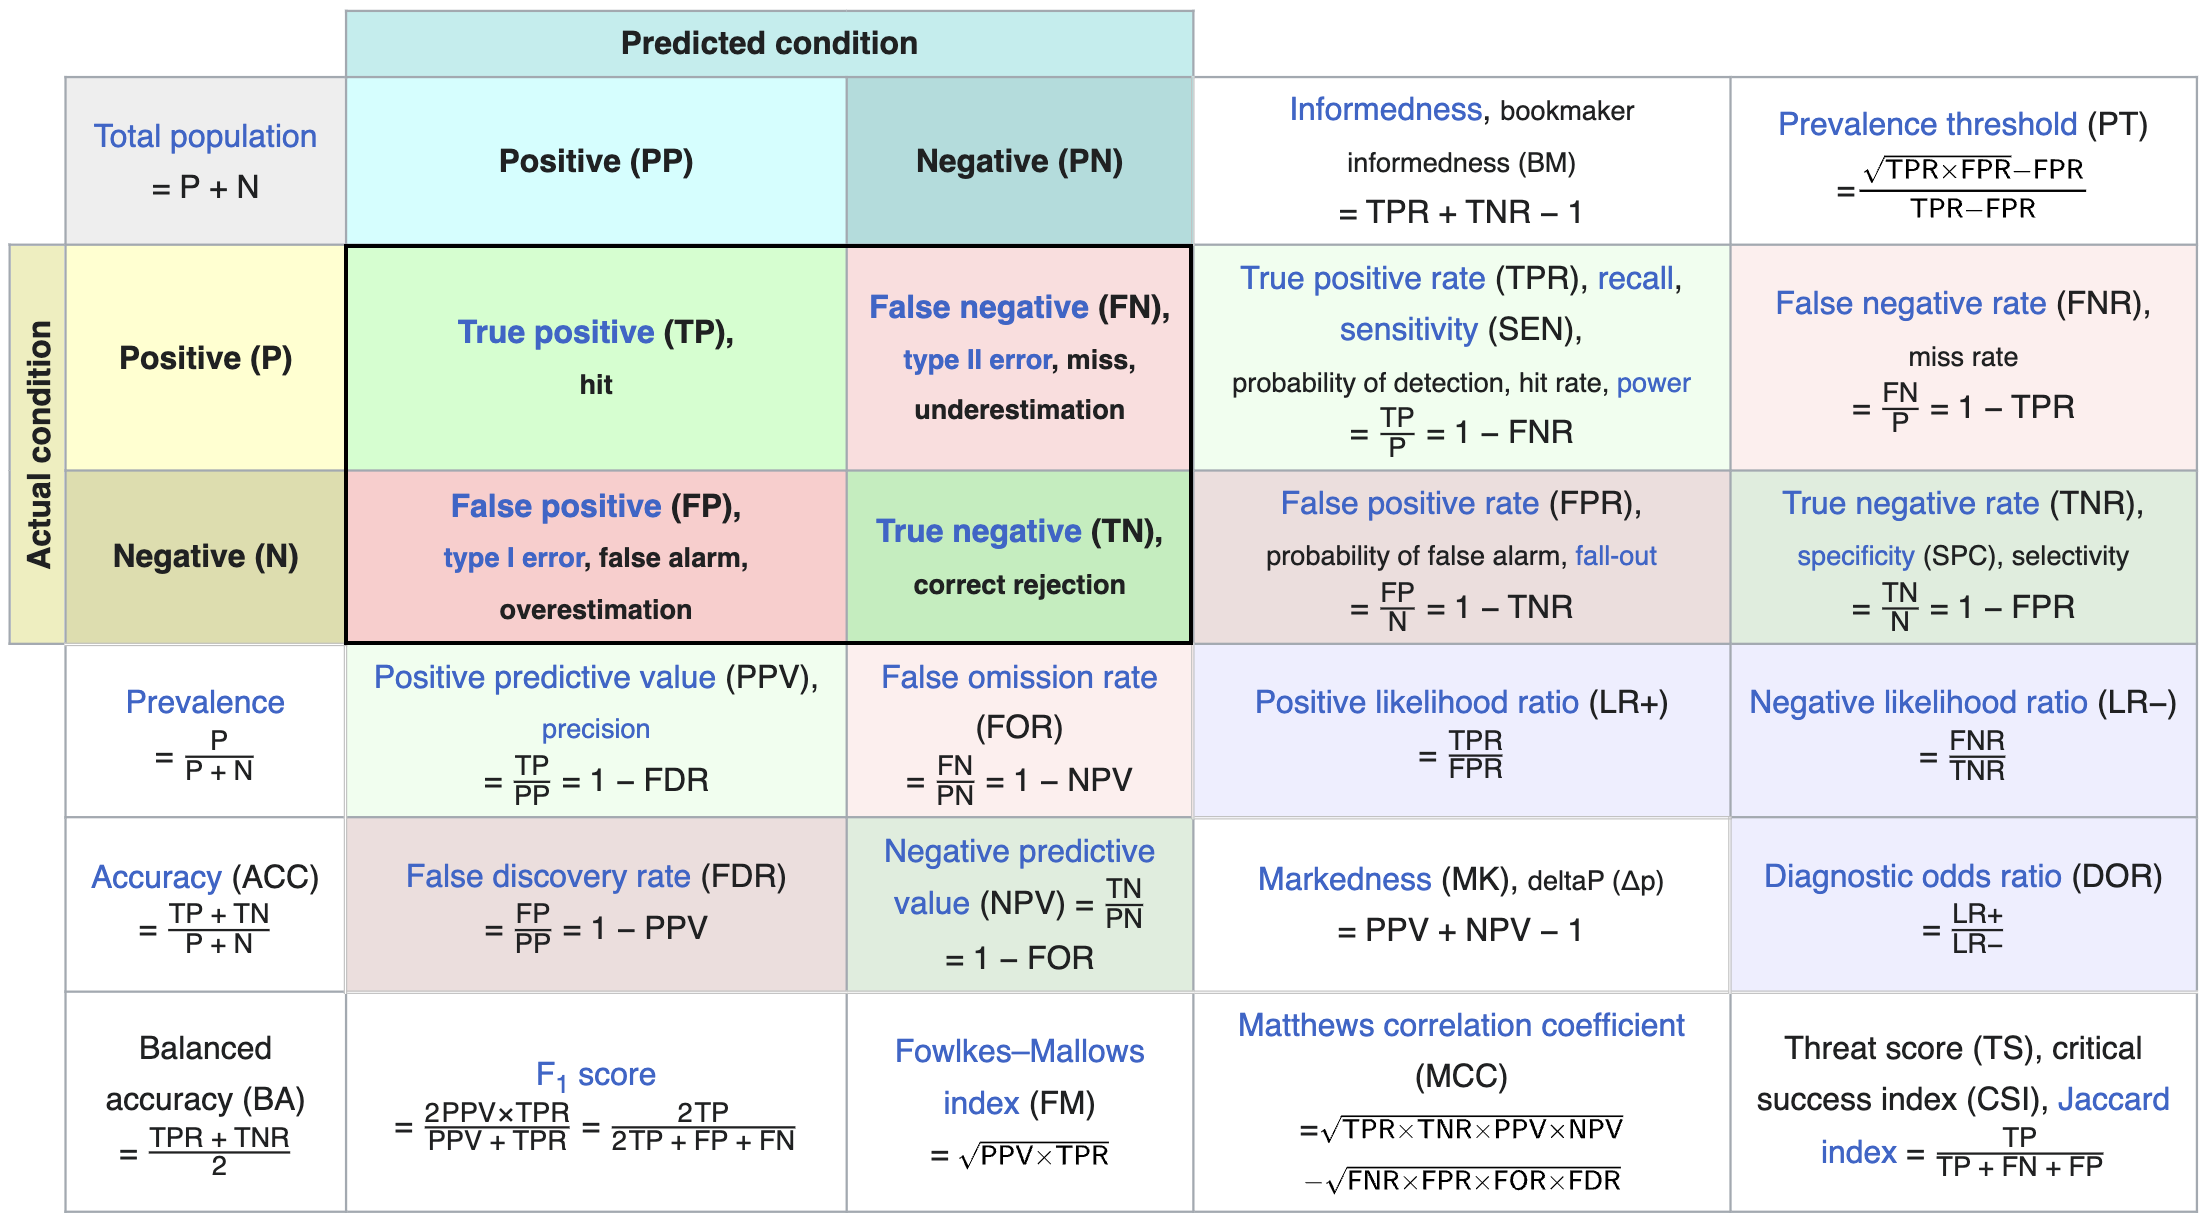
\includegraphics[width=\textwidth]{figs/confusionmtx.png}
%     \caption{Confusion matrix and the metrics defined on it}
%     {\footnotesize This table comes from Wikipedia (https://en.wikipedia.org/wiki/Confusion\_matrix).}
%     \label{fig:confusionmtx}
% \end{figure}

\begin{figure}[htpb]
    \centering
    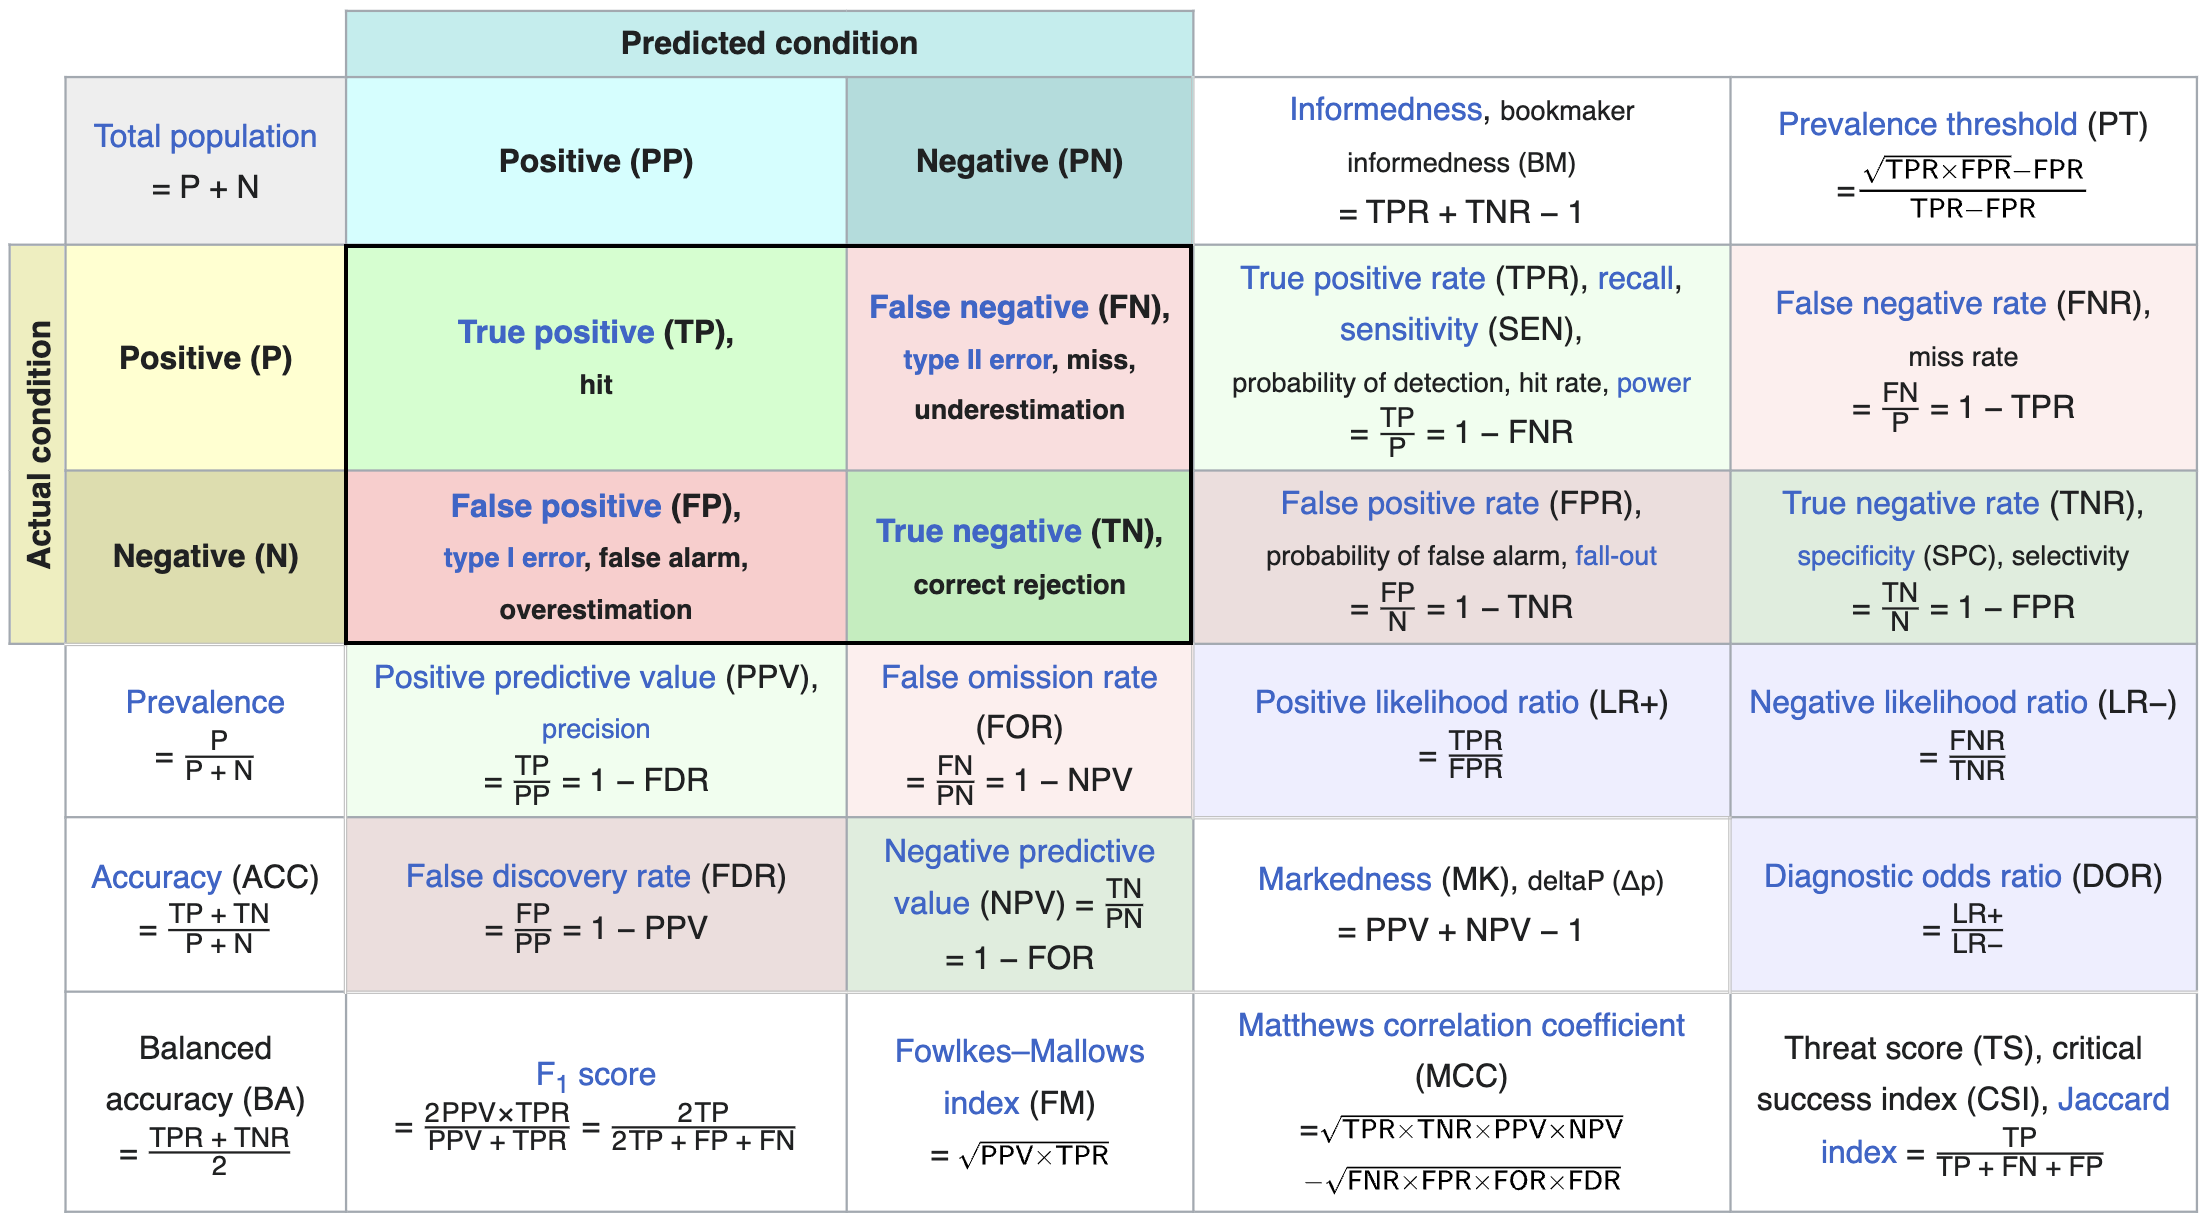
\includegraphics[width=\textwidth]{figs/confusionmtx.png}
    \caption{Confusion matrix and the metrics defined on it}
    {\footnotesize This table comes from Wikipedia (https://en.wikipedia.org/wiki/Confusion\_matrix).}
    \label{fig:confusionmtx}
\end{figure}

\textbf{Receiver operating characteristic (ROC) curves}: 
x-axis: FPR (1-Specificity) and y-axis: TPR (Recall or Sensitivity);
and \textbf{Precision-recall (PR) curves}:
x-axis: Recall and y-axis: Precision.
ROC curves (and the area under it, AUC) will not be unaffected by class imbalance,
while PR curves (and the area under \textit{interpolated} ones, AP) are sensitive to a large change in the absolute number in imbalance problem,
preferable when the shifting of absolute numbers are concerned, such as a ``negative'' is not well-defined.
 
\textbf{Huber loss}: equivalent to $\ell_2$ for errors smaller than $\delta$, 
and $\ell_1$for larger errors.
\begin{gather}
    \ell_\delta(h,a)=\left\{
    \begin{array}{ll}
        \frac{1}{2}(a-h)^2              & \text{if}~|a-h|\leq\delta\\
        \delta|a-h|-\frac{1}{2}\delta^2 & \text{if}~|a-h|>\delta
    \end{array}
    \right.
\end{gather}

\textbf{Kullback Leibler (KL) divergence}:
\begin{align}
    \infdiv{p}{q}
    \triangleq& \sum_{y\in\mathcal{Y}}p(y)\log\frac{p(y)}{q(y)}\\
    =& \underbrace{\sum_{y\in\mathcal{Y}}p(y)\log{p(y)}}_{-\mathbb{H}(p)}
        \underbrace{-\sum_{y\in\mathcal{Y}}p(y)\log{q(y)}}_{\mathbb{H}_\text{ce}(p,q)}.
\end{align}
Minimizing KL divergence between the fixed given $p$ and a $q$ is equal to find a $q$ minimizing the cross-entropy between $p$ and $q$.
$\log{\frac{p()y}{q(y)}}$ term can be quite sensitive to errors for low probability events,
so the \textbf{Brier score} an alternative
\begin{gather}
    \ell(p,q)\triangleq\frac{1}{C}\sum_{c=1}^C[q(y=c|\bm{x})-p(y=c|\bm{x})]^2
\end{gather}

\textbf{Bayes factor} for Bayesian hypothesis testing\unsure{
Recall the definition of marginal likelihood or evidence for a model $m$, 
$p(\mathcal{D}|m)=\int{p(\bm{\theta}|m)p(\mathcal{D}|\bm{\theta},m)}d\bm{\theta}$.
The model presented here is a family of distribution indexed by the parameter $\bm{\theta}$, 
so we need marginal likelihood for an average probability for family $m$ as feasible region of optimization.
}
\begin{gather}
    B_{1,0}\triangleq\frac{p(\mathcal{D}|M_1)}{p(\mathcal{D}|M_0)}
\end{gather}

\begin{table}[htbp]
    \centering
    \begin{tabular}{cl}
    \toprule
    Bayes factor $B_{0,1}$                      & Interpretation \\
    \midrule
    $(0,\frac{1}{100})$                         & Decisive evidence for $M_0$ \\
    $(\frac{1}{100},\frac{1}{10})$              & Strong evidence for $M_0$ \\
    $(\frac{1}{10},\frac{1}{3})$                & Moderate evidence for $M_0$ \\
    $(\frac{1}{3},1)$                           & Weak evidence for $M_0$ \\
    $(1,3)$                                     & Weak evidence for $M_1$ \\
    $(3,10)$                                    & Moderate evidence for $M_1$ \\
    $(10,100)$                                  & Strong evidence for $M_1$ \\
    $(100,\infty)$                              & Decisive evidence for $M_1$ \\
    \bottomrule
    \end{tabular}
    \caption{Jeffreys scale of evidence for interpreting Bayes factors}
    \label{tab:bayesfactor}
\end{table}

\textbf{Information criteria} ($D_m=|\bm{\theta}|$)
\begin{itemize}
    \item \textbf{Bayesian information criterion (BIC)}: 
    Gaussian approximation to the posterior $p(\bm{\theta}|\mathcal{D})$ with the assumptions of 
    {uniform prior ($p(\bm{\theta})\propto 1$) and iid of samples}.
    \begin{align}
        J_\text{BIC}(m)=&\log{p(\mathcal{D}|m)}\approx\log{p(\mathcal{D}|\hat{\bm{\theta}},m)-\frac{D_m}{2}\log{N}}\\
        \Rightarrow
        \mathcal{L}_\text{BIC}(m)=&-2\log{p(\mathcal{D}|\hat{\bm{\theta}},m)+D_m\log{N}}
    \end{align}
    
    \item \textbf{Akaike information criterion (AIC)}: 
    The regularization term independent of $N$ derives from a frequentist perspective.
    \begin{gather}
        \mathcal{L}_\text{AIC}(m)=-2\log{p(\mathcal{D}|\hat{\bm{\theta}},m)+2D_m}
    \end{gather}
    
    \item \textbf{Minimum description length (MDL)}:
    The bit length regularization term ($C(m)=-\log{p(m)}$) comes from the perspectives of communication cost.
    \begin{gather}
        \mathcal{L}_\text{MDL}(m)=-\log{p(\mathcal{D}|\hat{\bm{\theta}},m)+C(m)}
    \end{gather}
    
\end{itemize}

% \begin{figure}[htpb]
%     \centering
%     \begin{figure}[htpb]
    \centering
    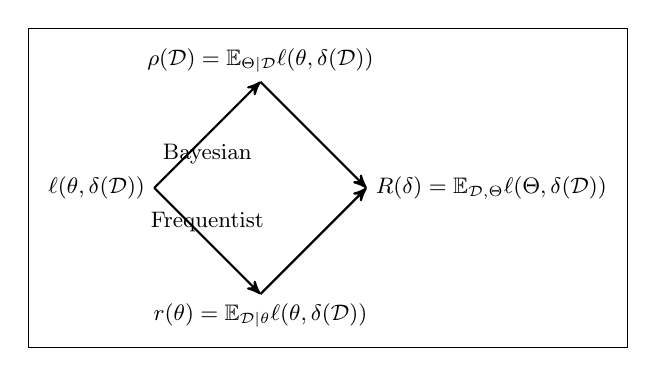
\begin{tikzpicture}[->,>=stealth',auto,node distance=3.5em,thick,show background rectangle]
    \tikzstyle{every node}=[font=\small,scale=0.9]
      \node[](anchor){};
      \node[left = of anchor]       (loss)  {$\ell(\theta,\delta(\mathcal{D}))$};
      \node[above = of anchor]          (bayes) {$\rho(\mathcal{D})=\mathbb{E}_{\Theta|\mathcal{D}}\ell(\theta,\delta(\mathcal{D}))$};
      \node[below = of anchor]         (freq)  {$r(\theta)=\mathbb{E}_{\mathcal{D}|\theta}\ell(\theta,\delta(\mathcal{D}))$};
      \node[right = of anchor]         (risk)  {$R(\delta)=\mathbb{E}_{\mathcal{D},\Theta}\ell(\Theta,\delta(\mathcal{D}))$};
      
      \draw[->] (loss.east)  --node[below]{Bayesian}     (bayes.south);
      \draw[->] (loss.east)  --node[above]{Frequentist}  (freq.north);
      \draw[->] (bayes.south) -- (risk.west);
      \draw[->] (freq.north)  -- (risk.west);
    \end{tikzpicture}
    \caption{risk from Bayesian and Frequentist perspective}
    \label{fig:riskbf}
\end{figure}
%     \caption{risk from Bayesian and Frequentist perspective}
%     \label{fig:riskbf}
% \end{figure}

\begin{figure}[htpb]
    \centering
    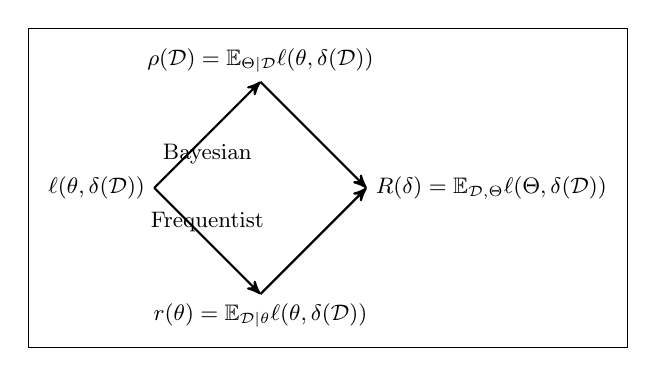
\begin{tikzpicture}[->,>=stealth',auto,node distance=3.5em,thick,show background rectangle]
    \tikzstyle{every node}=[font=\small,scale=0.9]
      \node[](anchor){};
      \node[left = of anchor]       (loss)  {$\ell(\theta,\delta(\mathcal{D}))$};
      \node[above = of anchor]          (bayes) {$\rho(\mathcal{D})=\mathbb{E}_{\Theta|\mathcal{D}}\ell(\theta,\delta(\mathcal{D}))$};
      \node[below = of anchor]         (freq)  {$r(\theta)=\mathbb{E}_{\mathcal{D}|\theta}\ell(\theta,\delta(\mathcal{D}))$};
      \node[right = of anchor]         (risk)  {$R(\delta)=\mathbb{E}_{\mathcal{D},\Theta}\ell(\Theta,\delta(\mathcal{D}))$};
      
      \draw[->] (loss.east)  --node[below]{Bayesian}     (bayes.south);
      \draw[->] (loss.east)  --node[above]{Frequentist}  (freq.north);
      \draw[->] (bayes.south) -- (risk.west);
      \draw[->] (freq.north)  -- (risk.west);
    \end{tikzpicture}
    \caption{risk from Bayesian and Frequentist perspective}
    \label{fig:riskbf}
\end{figure}

\textbf{Populaton risk}: if the true distribution $p^*{\bm{x}, \bm{y}}$ is known, 
then the risk of an estimator $f$ is 
\begin{gather}
    R(f,p^*)=R(f)\triangleq\mathbb{E}_{p^*(\bm{x},\bm{y})}\ell(\bm{y},f(\bm{x})).
\end{gather}
Of course, $p^*$ is unknown, 
but we can approximate it using the \textit{empirical distribution} with $N$ samples
and get \textbf{empirical risk}\unsure{
This distribution is discrete. 
If there are some new data point $(\bm{x},\bm{y})$ that haven't occur in dataset,
then, $p\mathcal{D}(\bm{x},\bm{y})=0$,
so it will need some smoothing method or, directly, use empirical expectation that averages over the observed data points.
Empirical risk minimization widely applied in training a deep learning model, 
and the hypothesis space $\mathcal{H}$ depends on the architecture of model.
}
\begin{gather}
    p_{\mathcal{D}}(\bm{x},\bm{y})
    \triangleq
    \frac{1}{|\mathcal{D}|}\sum_{(\bm{x}_n,\bm{y}_n)\in\mathcal{D}}\delta(\bm{x}-\bm{x}_n)\delta(\bm{y}-\bm{y}_n) \\
    R(f,\mathcal{D})
    \triangleq
    \mathbb{E}_{p_{\mathcal{D}}(\bm{x},\bm{y})}\ell(\bm{y},f(\bm{x}))=\frac{1}{N}\sum_{n=1}^N\ell(\bm{y}_n,f(\bm{x}_n))\\
    \hat{f}_\mathcal{D}=\argmin_{f\in\mathcal{H}}R(f,\mathcal{D}).
\end{gather}
Due to \uline{approximation of true distribution (from data)} and \uline{limitation of tractable hypothesis space (from model)}, 
there will exist errors between empirically optimal estimator $\hat{f}_\mathcal{D}$ and universally optimal estimator $f^{**}$
\begin{gather}
    f^{**}=\argmin_f R(f),~
    f^*=\argmin_{f\in\mathcal{H}} R(f),~
    f^*_{\mathcal{D}_\text{tr}}=\argmin_{f\in\mathcal{H}}R(f,\mathcal{D}_\text{tr})\\
    \mathbb{E}_{p^*}\left[R(f^*_{\mathcal{D}_\text{tr}})-R(f^{**})\right]
    =\underbrace{R(f^*)-R(f^{**})}_{\mathcal{E}_\text{app}(\mathcal{H})}
    +\underbrace{\mathbb{E}_{p^*}\left[R(f^*_{\mathcal{D}_\text{tr}})-R(f^*)\right]}_{\mathcal{E}_\text{est}(\mathcal{H,\mathcal{D}_\text{tr}})}\\
    % \mathbb{E}_{p^*}\left[R(f^*_{\mathcal{D}_\text{tr}})-R(f^*)\right]
    \mathcal{E}_\text{est}(\mathcal{H,\mathcal{D}_\text{tr}})
    = \mathbb{E}_{p_\text{tr}}\ell{(\bm{y},f^*_{\mathcal{D}_\text{tr}}(\bm{x}))}
    - \mathbb{E}_{p_\text{te}}\ell{(\bm{y},f^*_{\mathcal{D}_\text{tr}}(\bm{x}))} + \varepsilon_\text{gen}
\end{gather}
where 
$\mathcal{E}_\text{app}(\mathcal{H})$ is approximation error, 
$\mathcal{E}_\text{est}(\mathcal{H,\mathcal{D}_\text{tr}})$ is estimation/generalization error,
and $\varepsilon_\text{gen}$ is called generalization gap.

\textbf{Structural risk minimization}: minimized the regularized \textit{population} risk to pick a model of right complexity.
\begin{gather}
    \argmin_\lambda\min_{\bm{\theta}}\{R(\bm{\theta})+\lambda C(\bm{\theta})\}
\end{gather}
The empirical risk ignored the risk caused by unobserved data and underestimates the population risk,
and the minimization regularized empirical risk 
\begin{gather}
    R_\lambda(\bm{\theta},\mathcal{D})\triangleq R(\bm{\theta},\mathcal{D})+\lambda C(\bm{\theta})
\end{gather} 
always results in $\lambda=0$.
\begin{itemize}
    \item \textbf{cross-validation}\unsure{In the context of DL, $\lambda$ may be the number of training epochs.}
    \begin{gather}
        \hat{\bm{\theta}}_\lambda(\mathcal{D}_\text{tr})=\argmin_{\bm{\theta}}R_\lambda(\bm{\theta},\mathcal{D}_\text{tr}) \\
        R_\lambda^\text{val}\triangleq R(\hat{\bm{\theta}}_\lambda(\mathcal{D}_\text{tr}),\mathcal{D}_\text{val}),~\text{and}~
        R_\lambda^\text{cv}\triangleq\frac{1}{K}\sum_{k=1}^K{R(\hat{\bm{\theta}}(\mathcal{D}_{K\setminus k}),\mathcal{D}_k)} \\
        \hat{\lambda}=\argmin_\lambda R_\lambda^\text{cv} \\
        \hat{\bm{\theta}}=\argmin_{\bm{\theta}}R_{\hat{\lambda}}(\bm{\theta},\mathcal{D})
    \end{gather}\unsure{In real application, 
    the K model snapshots with the optimal $\hat{\lambda}$ during training process may be ensembled, 
    such as average the predictions,
    to a final model, instead of retrained on the entire dataset, 
    because of the additional cost in running time and resources of computation or storage.}
    \item \textbf{statistical learning theory}: Theorem \ref{thm:boundgenerror} tells us the gap between 
    empirical risk and population risk has an upper bound with some probability. 
    The prediction by the model that reach the upper bound is called \textbf{probability approximately correct},
    when the hypothesis class $\mathcal{H}$ is \textbf{PAC learnable}. 
\end{itemize}

\begin{theorem}\label{thm:boundgenerror}
    \textbf{{Upper bound of generalization risk}}\\
    For any data distribution $p^*$ and nay dataset $\mathcal{D}$ of size $N$ drawn from $p^*$,
    the probability that the \uline{generalization error of a binary classifier selected from a finite hypothesis class $\mathcal{H}$} 
    will be more that $\epsilon$.
    In the worst case, it is upper bounded as follows:
    \begin{gather}
        P\left(
            \max_{h\in\mathcal{H}}{|R(h)-R(h,\mathcal{D})|}>\epsilon
        \right)
        \leq 2\mathrm{dim}(\mathcal{H})\exp\{-2N\epsilon^2\}
    \end{gather}
    where $R(h,\mathcal{D})=\frac{1}{N}\sum_{n=1}^N \mathbb{I}(f(\bm{x}_n)\neq y_n)$ empirical risk, 
    $R(h)=\mathbb{E}_{p^*(\bm{x},y)}\mathbb{I}(f(\bm{x})\neq y)$ population risk, 
    and $\mathrm{dim}(\mathcal{H})=|\mathcal{H}|$.
    When the hypothesis class is infinite, we take $\mathrm{dim}(\mathcal{H})=\mathrm{dim}_\text{VC}(\mathcal{H})$,
    \textbf{VC dimension}, measuring the degrees of freedom of the hypothesis class.
    
    \textit{Remark}: the more data the less error; the larger hypothesis space the more error.
\end{theorem}


\subsection{Information Theory}

% \begin{figure}[htpb]
%     \centering
%     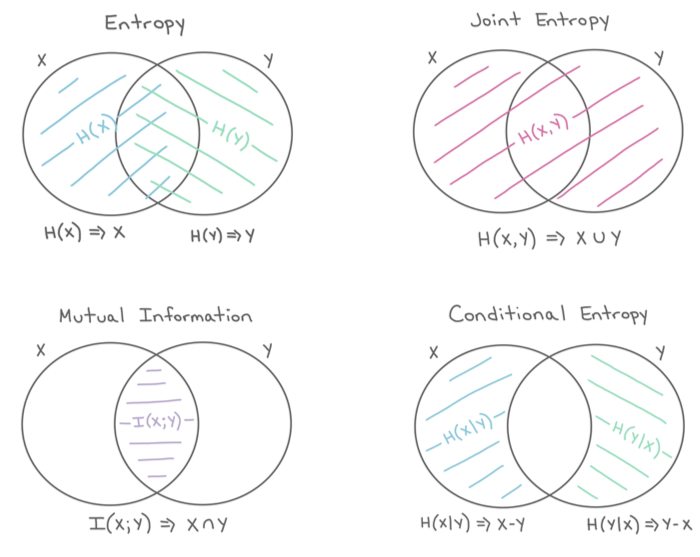
\includegraphics[width=0.6\textwidth]{figs/entropy.png}
%     \caption{The marginal entropy, joint entropy, conditional entropy and mutual information represented as information diagrams.}
%     \label{fig:entropy}
% \end{figure}

\begin{figure}[htpb]
    \centering
    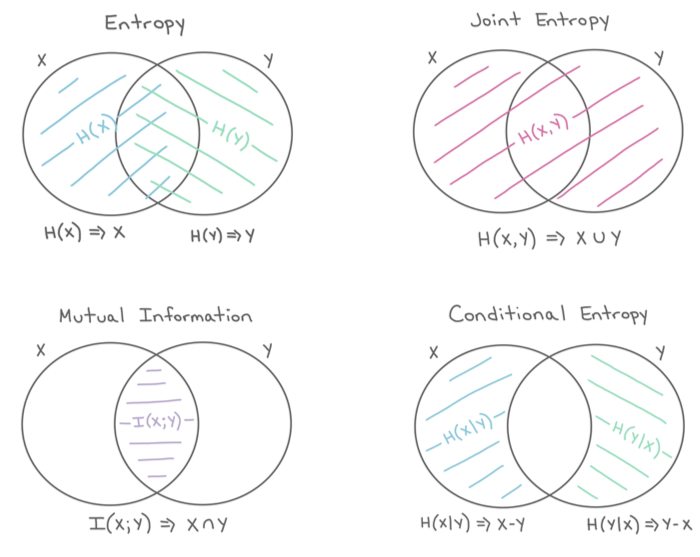
\includegraphics[width=0.6\textwidth]{figs/entropy.png}
    \caption{The marginal entropy, joint entropy, conditional entropy and mutual information represented as information diagrams.}
    \label{fig:entropy}
\end{figure}

\textbf{Cross entropy}: expected number of bits needed to compress some data
samples drawn from distribution $p$ using a code based on distribution $q$,
and the optimal code is reached by $q=p$, i.e., the entropy of $p$ \textbf{(Shannon's source coding theorem)}.
\begin{gather}
    \mathbb{H}(p,q)\triangleq-\sum_{k=1}^K p_k\log_2{q_k}\ge\mathbb{H}(p)
\end{gather}
The continuous version is called \textbf{differetial entropy}
\begin{gather}
    h(X)\triangleq-\int_{\mathcal{X}}p(x)\log{p(x)}dx,
\end{gather}
which can be negative and 
all real-valued quantities can be \uline{represented to finite precision}, 
says, \uline{$n$-bit} \textbf{quantization}, \unsure{Note it is not $B$-bin}
and the approximated discrete value's entropy will be $h(X)+n$. 
One simple approach to discretize is to bin the distribution based on its \uline{empirical quantiles} and the number of bins is determined by 
\begin{gather}
    B=N^\frac{1}{3}\frac{\max{D}-\min{D}}{3.5\sigma_\mathcal{D}}.
\end{gather}

\textbf{Joint entropy} of two random variables $X$ and $Y$
\begin{gather}
    \mathbb{H}(X,Y)=-\sum_{x\in\mathcal{X},y\in\mathcal{Y}}p(x,y)\log_2 p(x,y)\\
    0 \leq \max\{\mathbb{H}(X),\mathbb{H}(Y)\} \leq \mathbb{H}(X,Y) \leq \mathbb{H}(X) + \mathbb{H}(Y)
\end{gather}
where the right equality holds if $X$ \rotatebox{90}{$\models$} $Y$,
which says combining variables together does not make the entropy go down: you cannot
reduce uncertainty merely by adding more unknowns to the problem, you need to observe some data,
and if there is no information introduced by the additional unknowns, the system will reach the maximum chaos.

\textbf{Conditional entropy} of $Y$ given $X$ is the uncertainty we have in $Y$ after seeing $X$, averaged
over possible values for $X$
\begin{align}
    \mathbb{H}(Y|X)
    =& -\sum_{x\in\mathcal{X}}p(x)\sum_{y\in\mathcal{Y}}p(y|x)\log{p(y|x)} \\
    =& -\sum_{x\in\mathcal{X},y\in\mathcal{Y}}p(x,y)\log{\frac{p(x,y)}{p(x)}} \\
    =& \mathbb{H}(X,Y)-\mathbb{H}(X)
\end{align}
\begin{gather}
    0 \leq \mathbb{H}(Y|X) \leq \mathbb{H}(Y)
\end{gather}
where the left equality holds if $Y=f(X)$ where $f$ is deterministic, 
and the right equality holds if $X$ \rotatebox{90}{$\models$} $Y$,
which says that, \textit{on average}, conditioning on data never increases one’s uncertainty.
\begin{gather}
    \mathbb{H}(X_1,\cdots,X_n)=\sum_{i=1}^n{\mathbb{H}(X_i|X_1,\cdots,X_{i-1})}
\end{gather}

\textbf{Relative entropy} or KL divergence\unsure{
already introduced in Chapters 2 and 5.
} measures the (asymmetric) distance between two distributions, which can be interpreted as a lower bound on the number of bits (or ``extra number of bits'') needed to compress data coming from distribution $p$ based on $q$ as the basis of coding scheme.
\begin{align}
    \infdiv{p}{q}
    \triangleq& \sum_{y\in\mathcal{Y}}p(y)\log\frac{p(y)}{q(y)}\\
    =& \sum_{y\in\mathcal{Y}}p(y)\log{p(y)} -\sum_{y\in\mathcal{Y}}p(y)\log{q(y)} \\
    =& -\mathbb{H}(p) + \mathbb{H}_\text{ce}(p,q)
\end{align}

\begin{corollary}
    \textbf{Uniform distribution maximizes the entropy}\\
    $\mathbb{H}(X)\leq\log{|\mathcal{X}|}$, where $|\mathcal{X}|$ is the number of states for $X$, with equality iff $p(x)$ is uniform.
\end{corollary}
\begin{proof}
    Let $u(x)=\frac{1}{|\mathcal{X}|}$, then
    \begin{gather}
        0\leq\infdiv{p}{u}=\sum_{x\in\mathcal{X}}p(x)\log{\frac{p(x)}{q(x)}}=\log{|\mathcal{X}|-\mathbb{H}(X)}
    \end{gather}
\end{proof}

\textbf{Mutual information} measures the dependence of two random variables or the similarity of two distributions, which can serve as a generalized correlation coefficient
\begin{gather}
    \mathbb{I}(X;Y)\triangleq\infdiv{p(x,y)}{p(x)p(y)}
    =\sum_{x\in\mathcal{X}}\sum_{y\in\mathcal{Y}}p(x,y)\log\frac{p(x,y)}{p(x)p(y)}\geq 0
\end{gather}
where the right equality holds iff $X\vperp Y$ and MI approaches $\infty$ if $Y$ tells us an infinite amount of information about $X$.
\begin{align}
    \mathbb{I}(X;Y)
    =& \mathbb{H}(X)-\mathbb{H}(X|Y) \\
    =& \mathbb{H}(Y)-\mathbb{H}(Y|X) \\
    =& \mathbb{H}(X,Y)-\mathbb{H}(X|Y)-\mathbb{H}(Y|X) \\
    =& \mathbb{H}(X) + \mathbb{H}(Y) - \mathbb{H}(X,Y)
\end{align}
\textbf{Conditional mutual information} is the extra information that 
$X$ tells us about $Y$, excluding what we already knew about $Y$ given $Z$ alone.
\begin{align}
    \mathbb{I}(X;Y|Z)
    \triangleq& \mathbb{E}_{p(z)}[\mathbb{I}(X;Y)|Z] \\
    =& \mathbb{E}_{p(z,y,z)}\frac{p(x,y|z)}{p(x|z)p(y|z)} \\
    =& \mathbb{I}(Y;X,Z)-\mathbb{I}(Y;Z)
\end{align}
\textbf{Normalized mutual information (NMI)}: normalize the MI into $[0,1]$, served as ``modern correlation coefficient''
\begin{gather}
    \mathrm{NMI}(X,Y)=\frac{\mathbb{I}(X;Y)}{\min\{\mathbb{H}(X),\mathbb{H}(Y)\}}\in[0,1]
\end{gather}
which need a \uline{discretization technique} to make the \uline{computation tractable}:
\textbf{Maximal information coefficient}
\begin{gather}
    \mathrm{MIC}(X,Y)=\max_{G}\frac{I((X,Y)|_G)}{\log\|G\|}\approx\mathrm{NMI}(X,Y)
\end{gather}
where $G$ is a set of 2D grids, $(X,Y)|_G$ represents a 2D discretization of $X$ and $Y$,
$\|G\|\triangleq\min\{G_x,G_y\}$, $G_x$ is the number of grid cells in the $x$ direction, so be $G_y$.

\begin{theorem}
    \textbf{Data processing inequality}\\
    Suppose $X\to Y\to Z$ forms a Markov chain, so that $X\vperp Z|Y$.
    Then $\mathbb{I}(X;Y)\geq\mathbb{I}(X;Z)$.
\end{theorem}
\begin{proof}
    \begin{align}
        \mathbb{I}(X;Y,Z)
        =& \mathbb{I}(X;Z)+\mathbb{I}(X;Y|Z)\\
        =& \mathbb{I}(X;Y)+\mathbb{I}(X;Z|Y)
    \end{align}
    \begin{gather}
        X\vperp Z|Y\Rightarrow \mathbb{I}(X;Z|Y)=0\\
        \Rightarrow \mathbb{I}(X;Z)+\underbrace{\mathbb{I}(X;Y|Z)}_{\geq 0}=\mathbb{I}(X;Y) \\
        \Rightarrow \mathbb{I}(X;Y)\geq\mathbb{I}(X;Z)
    \end{gather}
    Similarly,
    \begin{gather}
        \mathbb{I}(Y;Z)\geq\mathbb{I}(X;Z)
    \end{gather}
\end{proof}


% \begin{framed}{\large
% TODO list of the following week
% \begin{itemize}
%     \item Finish the note organization work of Part II
%     \item Read Chapters 9 and 10
%     \item Course works
% \end{itemize}
% }
% \end{framed}





% ############################### WK 3 #######################################

% \setcounter{section}{2}
% \setcounter{subsection}{6}
% \begin{center}
% \textit{Chapter 7 Linear Algebra \& Chapter 8 Optimization $\S$ 1-5.}
% \end{center}

% % \subsection{Decision Theory}

% \subsection{Information Theory}


\setcounter{subsection}{6}
\subsection{Linear Algebra}

\begin{table}[htpb]
    \centering
    \begin{tabular}{rp{32em}}
        \toprule
        Terminology & Brief definition\\
        \midrule
        \textbf{span} of vectors &  $\text{span}(\{\bm{x}_1,\cdots,\bm{x}_n\})\triangleq\left\{\bm{v}:\bm{v}=\sum_{i=1}^n\alpha_i\bm{x}_i,\alpha_i\in\mathbb{R}\right\}$\\
        \textbf{range} of a matrix & $\text{range}(\mathbf{A})\triangleq\{\bm{v}=\mathbf{A}\bm{x}\}$, column space \\ 
        \textbf{nullspace} of a matrix & $\text{nullspace}(\mathbf{A})\triangleq{\{\bm{x}:\mathbf{A}\bm{x}=\bm{0}\}}$\\
        \textbf{projection} & $\text{Proj}(\bm{y};\{\bm{x}_1,\cdots,\bm{x}_n\})=\argmin_{\bm{v}\in\text{span}(\{\bm{x}_1,\cdots,\bm{x}_n\})}\|\bm{y}=\bm{v}\|_2$ 
        or if $\mathbf{A}$ full rank in columns $\text{Proj}(\bm{y};\mathbf{A})=\mathbf{A}(\mathbf{A}^T\mathbf{A})^{-1}\mathbf{A}^T\bm{y}$ \\
        \textbf{max-norm} and \textbf{0-norm} & $\|\bm{x}\|_\infty=\max|x_i|$ and $\|\bm{x}\|_0=\sum_{i=1}^n\mathbb{I}(x_i\neq 0)$\\
        \bottomrule
    \end{tabular}
    \caption{Gleanings of linear algebra concepts}
    \label{tab:linalgc}
\end{table}

\textbf{Induced norm} of a matrix:\unsure{
recall that the \textbf{norm of a vector} is a measure of the vector's length or magnitude
and singular value of a matrix is }
The maximum response of a linear function by unite-norm input
\begin{gather}
    \|\mathbf{A}\|_p=\max_{\bm{x}\neq\bm{0}}\frac{\|\mathbf{A}\bm{x}\|_p}{\|\bm{x}\|_p}=\max_{\|\bm{x}\|_p=1}\|\mathbf{A}\bm{x}\|_p
\end{gather}


% \subsection{Optimization}

% \begin{figure}[htpb]
    \centering
    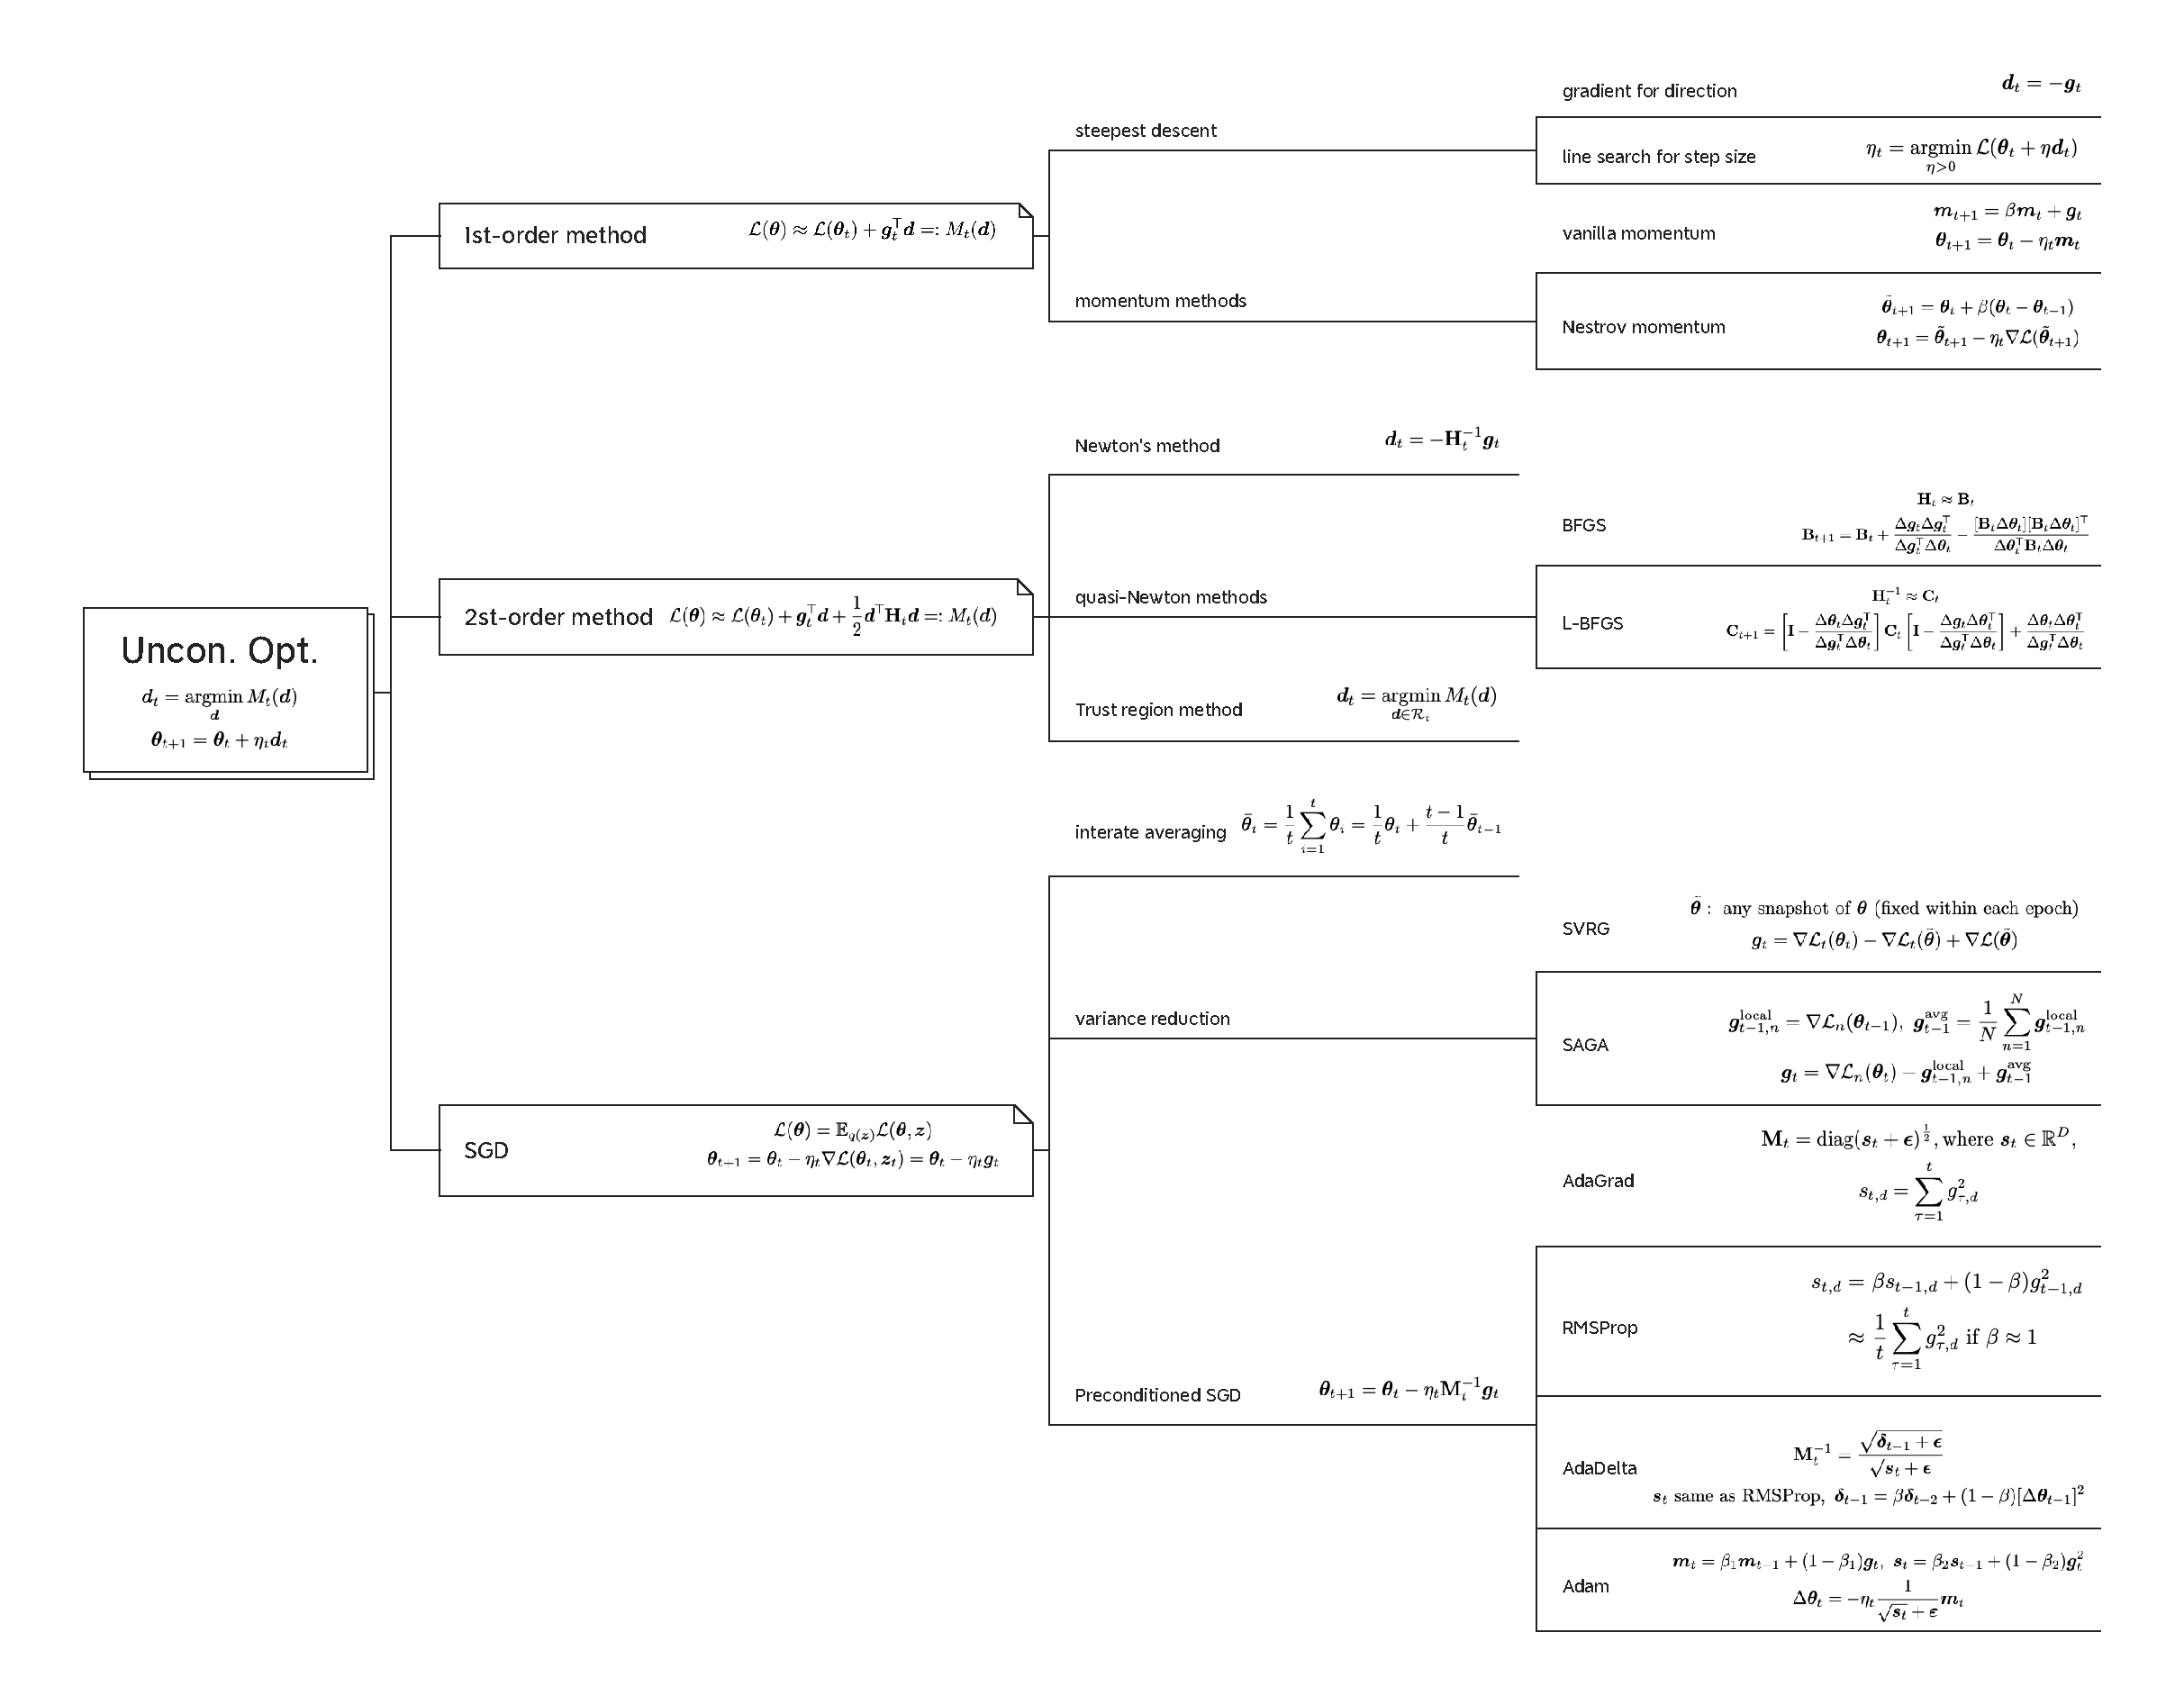
\includegraphics[width=\textwidth]{figs/unconopt.pdf}
    \caption{Solutions for unconstrained optimization updating strategies}
    {\footnotesize there are approximation methods for $M_t(\bm{d})$ and $\bm{d}_t$.
    \textbf{BFGS}: Broyden, Fletcher, Goldfarb and Shanno;
    \textbf{L-BFGS}: limited memory BFGS;
    \textbf{SGD}: Stochastic Gradient Descent;
    \textbf{SVRG}: Stochastic Variance Reduced Gradient;
    \textbf{SAGA}: Stochastic Averaged Gradient Accelerated;
    \textbf{AdaGrad}: ADAptive Gradient;
    \textbf{RMSProp}: Root Mean Squared resilient PROPagation;
    \textbf{Adam}: Adaptive moment estimation.
    }
    
    \label{fig:unconopt}
\end{figure}

% \textit{Handwriting notes were put on the book directly.\\
% To be continue...}

% \begin{framed}{\large
% TODO list of the following two weeks
% \begin{itemize}
%     \item Organize the reading notes and read the remained $\S$ 8.6-8.8, especially EM algorithm;
%     \item Read Chapters 5 and 6 (Decision Theory $\And$ Information Theory);
%     \item Course works:
%     \begin{enumerate}
%         \item homework of Linear Model (5030),
%         \item Read reference books of Multivariable Analysis (5020),
%         \item Exercises of Probability $\And$ Inference.
%     \end{enumerate}
% \end{itemize}
% }
% \end{framed}





% ############################### WK 6 #######################################

% \setcounter{section}{3}
% \begin{center}
% \textit{Chapter 9 Linear Discriminant Analysis \& Chapter 10 Logistic Regression.}
% \end{center}

\section{Linear Models}

\begin{quote}
    \citep{pml1Book} -- Chapters 9-12.
\end{quote}

\subsection{Linear Discriminant Analysis}

\textbf{Generative classifier}: 
modeling that the features are generated from \textbf{class conditional density} $p(\bm{x}|y=c;\bm{\theta})$
\begin{gather}
    % p(y)=\mathrm{Cat}(y|\bm{\pi})\\
    p(y=c|\bm{x};\bm{\theta})=
    \frac{{\color{red}p(\bm{x}|y=c;\bm{\theta})}{\color{blue}p(y=c;\bm{\theta})}}
    {\sum_{c'\in\mathcal{C}}p(\bm{x}|y=c';\bm{\theta})p(y=c';\bm{\theta})}\\
    % \underbrace{
    % \log{p(y=c|\bm{x};\bm{\theta})}=[\bm{w}(\bm{\theta})]^\mathsf{T}\bm{x}+\text{const}}_\text{LDA}
    % ~\text{for some special}~p(\bm{x}|y=c;\bm{\theta})
\end{gather}
\textbf{discriminative classifier}: classifying the samples directly by modeling $p(y|\bm{x},\bm{\theta})$ directly.
\begin{itemize}
    \item \textbf{Gaussian discriminant analysis} $p(\bm{x}|y=c;\bm{\theta})=\mathcal{N}(\bm{x}|\bm{\mu}_c,\bm{\Sigma}_c)$
\end{itemize}\unsure{
\color{red}What special class conditional density?
}

\textbf{Gaussian discriminant analysis}: 
\begin{align}
    p(y) =&~ \mathrm{Cat}(y|\bm{\pi})\\
    p(\bm{x}|y=c;\bm{\theta})
    =&~ \mathcal{N}(\bm{x}|\bm{\mu}_c,\bm{\Sigma}_c)\\
    =&~ (2\pi)^{-\frac{D}{2}}|\bm{\Sigma}_c|^{-\frac{1}{2}}\exp\left\{
        -\frac{1}{2}(\bm{x}-\bm{\mu}_c)^\mathsf{T}\bm{\Sigma}_c^{-1}(\bm{x}-\bm{\mu}_c)
    \right\}
\end{align}

\textbf{Quadratic decision boundaries}: 
for $\text{unspecified}~\bm{\Sigma}_c$
\begin{align}
    \log{p(y=c|\bm{x},\bm{\theta})}
    =&~ \log{\pi_c}-\frac{1}{2}\log|2\pi\bm{\Sigma}_c| \\
      -&~ \boxed{\frac{1}{2}(\bm{x}-\bm{\mu}_c)^\mathsf{T}\bm{\Sigma}_c^{-1}(\bm{x}-\bm{\mu}_c)}
      + \text{const}
\end{align}

\textbf{Linear decision boundaries}: 
for $\bm{\Sigma}_c=\bm{\Sigma}~(\text{shared}~\bm{\Sigma})$
\begin{align}
    \log{p(y=c|\bm{x},\bm{\theta})}
    =&~ \overbrace{
        \log{\pi_c} - \frac{1}{2}\bm{\mu}_c^\mathsf{T}\bm{\Sigma}^{-1}\bm{\mu}_c
    }^{\gamma_c} \\
    +&~ \boxed{
        \bm{x}^\mathsf{T}\underbrace{\bm{\Sigma}^{-1}\bm{\mu}_c}_{\bm{\beta}_c}
    }
    + \underbrace{
        \text{const} - \frac{1}{2}\bm{x}^\mathsf{T}\bm{\Sigma}^{-1}\bm{x}
    }_{\kappa}
\end{align}

\textbf{Logistic Regression}:
\begin{align}
    p(y=c|\bm{x},\bm{\theta})
    =&~ \frac{\exp\{\bm{\beta}_c^\mathsf{T}\bm{x}+\gamma_c\}}{\sum_{c'}\exp\{\bm{\beta}_{c'}^\mathsf{T}\bm{x}+\gamma_{c'}\}} \\
    =&~ \frac{\exp\{\bm{w}_c^\mathsf{T}[1,\bm{x}]\}}{\sum_{c'}\exp\{\bm{w}_{c'}^\mathsf{T}[1,\bm{x}]\}}
\end{align}
If $C=2$, we have 
\begin{align}
    p(y=1|\bm{x},\bm{\theta}) 
    =&~ \sigma\left((\bm{\beta}_1-\bm{\beta}_0)^\mathsf{T}\bm{x}+(\gamma_1-\gamma_0)\right)\\
    =&~ \sigma(\bm{w}^\mathsf{T}(\bm{x}-\bm{x}_0))\\
    \bm{w} =&~ \bm{\beta}_1-\bm{\beta}_0 = \bm{\Sigma}^{-1}(\bm{\mu}_1-\bm{\mu}_0) \\
    \bm{x}_0 =&~ \frac{1}{2}(\bm{\mu}_1 + \bm{\mu}_0) 
        - (\bm{\mu}_1 - \bm{\mu}_0)
        \frac{\log(\pi_1/\pi_0)}
        {(\bm{\mu}_1 - \bm{\mu}_0)^\mathsf{T}\bm{\Sigma}^{-1}(\bm{\mu}_1 - \bm{\mu}_0)}
\end{align}


\textbf{MLE}:
\begin{align}
    \hat{\bm{\mu}}_c =&~ \frac{1}{N_{\mathcal{D}}}\sum_{n:y_n=c}\bm{x}_n \\
    \hat{\bm{\Sigma}}_c =&~ \frac{1}{N_{\mathcal{D}_c}}\sum_{n:y_n=c}
    \left(\bm{x}_n-\hat{\bm{\mu}}_c\right)\left(\bm{x}_n-\hat{\bm{\mu}}_c\right)^\mathsf{T}
\end{align}

\textbf{Tied covariance}:
\begin{align}
    \hat{\bm{\Sigma}}
    =&~ \frac{1}{N_{\mathcal{D}}}\sum_{c=1}^C\sum_{n:y_n=c}
    \left(\bm{x}_n-\hat{\bm{\mu}}_c\right)\left(\bm{x}_n-\hat{\bm{\mu}}_c\right)^\mathsf{T} \\
    =&~ \sum_{c=1}^C\frac{N_{\mathcal{D}_c}}{N_{\mathcal{D}}}\hat{\bm{\Sigma}}_c
\end{align}

\textbf{MAP estimation} for \textbf{regularized discriminant analysis} (RDA):
\begin{align}
    \hat{\bm{\Sigma}}_{\text{map}} = \lambda\mathrm{diag}(\hat{\bm{\Sigma}}_{\text{mle}}) + (1-\lambda)\hat{\bm{\Sigma}}_{\text{mle}}
\end{align}

\textbf{Nearest centroid classifier}
\begin{align}
    \hat{y}(\bm{x})=\argmin_{c}(\bm{x}-\bm{\mu}_c)^\mathsf{T}\bm{\Sigma}^{-1}(\bm{x}-\bm{\mu}_c)
\end{align}
\subsection{Logistic Regression}

\textit{Notes of Chapter 9 \& 10 are still under going.\\
To be continue...}

\begin{framed}{\large
TODO list of the following week
\begin{itemize}
    \item Organize notes for Chapters 9 \& 10;
    \item Read Chapters 11 \& 12
\end{itemize}
}
\end{framed}


% ############################### WK 7 #######################################

% \setcounter{section}{3}
% \begin{center}
% \textit{Chapter 11 Linear Regression \& Chapter 12 Generalized Linear Model.}
% \end{center}

% \subsection{Linear Regression}

\subsection{Generalized Linear Model}



% \begin{framed}{\large
% TODO list of the following week
% \begin{itemize}
%     \item Read Chapters 13 \& 14;
% \end{itemize}
% }
% \end{framed}



\listnotes
\bibliography{ref}

\end{document}
